
\documentclass[11pt]{article}
\usepackage{amsmath, amssymb, graphicx, outline, float, cite, color}
\usepackage{lineno}

%%%%%%%%%%%%%%%%%%%%%%%%%%%%%%%%%%%%%%%%%
% Wenneker Article
% Structure Specification File
% Version 1.0 (28/2/17)
%
% This file originates from:
% http://www.LaTeXTemplates.com
%
% Authors:
% Frits Wenneker
% Vel (vel@LaTeXTemplates.com)
%
% License:
% CC BY-NC-SA 3.0 (http://creativecommons.org/licenses/by-nc-sa/3.0/)
%
%%%%%%%%%%%%%%%%%%%%%%%%%%%%%%%%%%%%%%%%%

%----------------------------------------------------------------------------------------
%	PACKAGES AND OTHER DOCUMENT CONFIGURATIONS
%----------------------------------------------------------------------------------------

\usepackage[english]{babel} % English language hyphenation

\usepackage{microtype} % Better typography

\usepackage{amsmath,amsfonts,amsthm} % Math packages for equations

\usepackage[svgnames]{xcolor} % Enabling colors by their 'svgnames'

\usepackage[hang, small, labelfont=bf, up, textfont=it]{caption} % Custom captions under/above tables and figures

\usepackage{booktabs} % Horizontal rules in tables

\usepackage{lastpage} % Used to determine the number of pages in the document (for "Page X of Total")

\usepackage{graphicx} % Required for adding images

\usepackage{enumitem} % Required for customising lists
\setlist{noitemsep} % Remove spacing between bullet/numbered list elements

\usepackage{sectsty} % Enables custom section titles
\allsectionsfont{\usefont{OT1}{phv}{b}{n}} % Change the font of all section commands (Helvetica)

%----------------------------------------------------------------------------------------
%	MARGINS AND SPACING
%----------------------------------------------------------------------------------------

\usepackage{geometry} % Required for adjusting page dimensions

\geometry{
	top=2cm, % Top margin
	bottom=2cm, % Bottom margin
	left=3cm, % Left margin
	right=3cm, % Right margin
	includehead, % Include space for a header
	includefoot, % Include space for a footer
	%showframe, % Uncomment to show how the type block is set on the page
}

\setlength{\columnsep}{7mm} % Column separation width

%----------------------------------------------------------------------------------------
%	FONTS
%----------------------------------------------------------------------------------------

\usepackage[T1]{fontenc} % Output font encoding for international characters
\usepackage[utf8]{inputenc} % Required for inputting international characters

\usepackage{XCharter} % Use the XCharter font

%----------------------------------------------------------------------------------------
%	HEADERS AND FOOTERS
%----------------------------------------------------------------------------------------

\usepackage{fancyhdr} % Needed to define custom headers/footers
\pagestyle{fancy} % Enables the custom headers/footers

\renewcommand{\headrulewidth}{0.0pt} % No header rule
\renewcommand{\footrulewidth}{0.4pt} % Thin footer rule

\renewcommand{\sectionmark}[1]{\markboth{#1}{}} % Removes the section number from the header when \leftmark is used

%\nouppercase\leftmark % Add this to one of the lines below if you want a section title in the header/footer

% Headers
\lhead{} % Left header
\chead{\textit{\thetitle}} % Center header - currently printing the article title
\rhead{} % Right header

% Footers
\lfoot{} % Left footer
\cfoot{} % Center footer
\rfoot{\footnotesize Page \thepage\ of \pageref{LastPage}} % Right footer, "Page 1 of 2"

\fancypagestyle{firstpage}{ % Page style for the first page with the title
	\fancyhf{}
	\renewcommand{\footrulewidth}{0pt} % Suppress footer rule
}

%----------------------------------------------------------------------------------------
%	TITLE SECTION
%----------------------------------------------------------------------------------------

\newcommand{\authorstyle}[1]{{\large\usefont{OT1}{phv}{b}{n}\color{DarkRed}#1}} % Authors style (Helvetica)

\newcommand{\institution}[1]{{\footnotesize\usefont{OT1}{phv}{m}{sl}\color{Black}#1}} % Institutions style (Helvetica)

\usepackage{titling} % Allows custom title configuration


%\newcommand{\HorRule}{\color{DarkGrey}\rule{\linewidth}{1pt}} % Defines the gold horizontal rule
\newcommand{\HorRule}{\color{DarkGoldenrod}\rule{\linewidth}{1pt}} % Defines the gold horizontal rule
 
\pretitle{
	\vspace{-30pt} % Move the entire title section up
	\HorRule\vspace{10pt} % Horizontal rule before the title
	\fontsize{20}{18}\usefont{OT1}{phv}{b}{n}\selectfont % Helvetica
	\color{DarkRed} % Text colour for the title and author(s)
}

\posttitle{\par\vskip 15pt} % Whitespace under the title

\preauthor{} % Anything that will appear before \author is printed

\postauthor{ % Anything that will appear after \author is printed
	\vspace{10pt} % Space before the rule
	\par\HorRule % Horizontal rule after the title
	\vspace{20pt} % Space after the title section
}

%----------------------------------------------------------------------------------------
%	ABSTRACT
%----------------------------------------------------------------------------------------

\usepackage{lettrine} % Package to accentuate the first letter of the text (lettrine)
\usepackage{fix-cm}	% Fixes the height of the lettrine

\newcommand{\initial}[1]{ % Defines the command and style for the lettrine
	\lettrine[lines=3,findent=4pt,nindent=0pt]{% Lettrine takes up 3 lines, the text to the right of it is indented 4pt and further indenting of lines 2+ is stopped
		%\color{DarkRed}% Lettrine colour
		\color{DarkGoldenrod}% Lettrine colour
		{#1}% The letter
	}{}%
}

\usepackage{xstring} % Required for string manipulation

\newcommand{\lettrineabstract}[1]{
	\StrLeft{#1}{1}[\firstletter] % Capture the first letter of the abstract for the lettrine
	\initial{\firstletter}\textbf{\StrGobbleLeft{#1}{1}} % Print the abstract with the first letter as a lettrine and the rest in bold
}

%----------------------------------------------------------------------------------------
%	BIBLIOGRAPHY
%----------------------------------------------------------------------------------------

%\usepackage[backend=bibtex,style=authoryear,natbib=true]{biblatex} % Use the bibtex backend with the authoryear citation style (which resembles APA)

%\addbibresource{example.bib} % The filename of the bibliography

%\usepackage[autostyle=true]{csquotes} % Required to generate language-dependent quotes in the bibliography



\graphicspath{ {Figs/} }

\usepackage[normalem]{ulem}
\usepackage[T1]{fontenc}
\usepackage[utf8]{inputenc}
\usepackage{authblk}
\usepackage{framed}

\newcommand{\tcr} { \textcolor{red} }
\newcommand{\tcb} { \textcolor{blue} }


\title{
Modeling the competing effects of the immune system and EMT on epithelial cancers
}

\author{Daniel R. Bergman$^{1}$,
Matthew K. Karikomi\,$^{1}$,
Min Yu\,$^{4}$,
Qing Nie\,$^{1,2,*}$
and Adam L. MacLean\,$^{1,3,*}$
}
\affil{
  $^1$Department of Mathematics, University of California, Irvine,  Irvine, CA 92697, USA \\
  $^2$Department of Cell and Developmental Biology, University of California, Irvine, Irvine, CA 92697, USA \\
  $^3$Department of Biological Sciences, University of Southern California, Los Angeles, CA 90089, USA \\
  $^4$Department of Stem Cell \& Regenerative Medicine, Keck School of Medicine, University of Southern California, Los Angeles, CA 90033, USA \\
  $^*$Correspondence:  qnie@uci.edu (QN); macleana@usc.edu (ALM).
}

\renewcommand\Authands{ and }

\date{}


\begin{document}
\maketitle


\section*{Abstract}
During progression from carcinoma in situ to an invasive tumor, the immune system is engaged in complex sets of interactions with various tumor cells.
Inflammation has particularly significant effects on gastrointestinal and pancreatic tumors.
Moreover, tumor cell plasticity can significantly alter disease trajectories via epithelial-to-mesenchymal transition (EMT).
Several of the same pathways that regulate EMT are involved in tumor-immune interactions, yet little is known about the mechanisms and consequences of these regulatory processes.
Here we introduce a multiscale evolutionary model to describe the interplay between tumor-immune-EMT interactions and their impact on epithelial cancers.
Through {\em in silico} analysis of large patient cohorts, we found controllable regimes that maximize invasion-free survival.
Delaying progression depended crucially on properties of the mesenchymal tumor cell phenotype: its growth rate and its immune-evasiveness.
We performed analysis of pancreatic cancer data from The Cancer Genome Atlas to compare clinical measurements with model predictions.
We found that association with EMT worsened the invasion-free survival probabilities of inflammation-associated cancer.
These results offer novel means to delay disease progression by regulating properties of EMT, and demonstrate the importance of studying cancer-immune interactions in light of EMT.

\linenumbers

%%%%%%%%%%%%%%%%%%%%%%%
%                    INTRODUCTION                    %
%%%%%%%%%%%%%%%%%%%%%%%


\section{Introduction}
The majority of deaths from cancer are due to metastasis of the disease \cite{dillekas}. It is thus of critical importance to understand better the progression from in situ to invasive disease. Underlying this progression are genetic and epigenetic events, including mutations in pathways critical to the success of the cancer cell (driver mutations) \cite{ryan2016hallmarks}. These pathways include cell proliferation, apoptosis, and immunogenicity.
\par 
Cancer and the immune system interact in myriad ways. Beyond direct tumor-immune cell interactions, the immune system modulates the tumor microenvironment (TME): responding to local inflammatory signals, targeting mutated cells, and eradicating tumor cells to potentially restore homeostasis in a local context \cite{de2006paradoxical}.
Recent breakthroughs in the field of immunotherapy are beginning to produce therapies that have had a significant impact on patient health and survival \cite{pardoll2012blockade,restifo2012adoptive}.
\par 
Tumor cells interact with the immune system by initiating a sequence of events that results in the activation of the adaptive immune response. This is accomplished by the presentation of antigens recognized by innate immune cells that are transported to lymph nodes where T cells (and other components) can be activated \cite{schreiber11_cancer}. The tumor also engages in cellular processes that indirectly shape the TME, for example by releasing transforming growth factor beta (TGF-$\beta$), thus shifting the TME towards a tumor-supportive environment by enhancing immunosuppression via activation of T regulatory cells (Tregs) \cite{schreiber11_cancer}.
\par
The effects of the immune system on a tumor can be broadly summarized into two modules. The cytotoxic branch of the immune system, such as natural killer cells (NKs) and cytotoxic T cells (CTLs), seek out and lyse tumor cells.
Upon carrying out their effector functions, these cytotoxic cells lose efficacy or deactivate entirely \cite{finn12_immunooncology-1}.
The regulatory branch of the immune system (Tregs and other factors), inhibits the effective functioning of the cytotoxic branch \cite{ruffell2010lymphocytes}.
%In addition, the immune system plays important regulatory roles in premalignant tissue, where
Inflammation can also increase the probability of progression (and/or decrease the time to invasion), with some of the most pronounced effects seen for tumors originating in gastrointestinal and pancreatic tissues \cite{hu10_inflammationinduced, balkwill01_inflammation}.
Recent work has shown, contrary to these typical effects of inflammation that under certain conditions inflammation may not be oncogenic but rather onco-protective \cite{guo17_multiscale}.
\par
Epithelial-to-mesenchymal transition (EMT) describes a reversible process by which cells with an epithelial phenotype transition into cells with a mesenchymal phenotype.
While epithelial cells are in part defined by their adhesion to neighbors, mesenchymal cells show much greater ranges of motility, and may display stem-like properties \cite{nieto2016emt}, although controversy regarding `stemness' and EMT remains \cite{nie18_stem, sha19_intermediate}.  
Recent work has shown that -- rather than being a binary process -- at least two stable intermediate states exist on the EMT axis \cite{hong2015ovol2, jolly15_coupling}.
Ongoing investigations into the plasticity and stability of EMT overlap with discussions elsewhere, e.g. of discrete vs. continuous processes during cell differentiation \cite{moris16_transition}.
Intermediate states have emerged as a central mechanism by which cell fates (and the noise inherent within them) can be controlled \cite{maclean18_exploring, ta16_controlling, rackauckas18_meanindependent}. 
\par 
While EMT has for some time been assumed to impact metastasis, more recently EMT-related phenotypes have been linked to other aspects of tumor progression \cite{nieto2016emt,peinado2007snail}.
TGF-$\beta$ is a master regulator of EMT \cite{lim2012epithelial}, linking it to the signaling networks involved in tumor-mediated immune responses, since Tregs release TGF-$\beta$ upon arriving at the tumor site\cite{terry2017new}. 
There is evidence directly linking Treg-secreted TGF-$\beta$ with EMT in hepatocellular carcinoma\cite{shi2019cd4+}.
Thus, even by considering only a single signaling factor, we find these three components (the tumor, the immune system, and EMT) to be linked. It therefore strikes us as a priority to develop models to understand how interactions between each of these three components affect cancer incidence and progression.
\par
Two features of the mesenchymal phenotype are of particular relevance in the context of cancer and the immune system: i) mesenchymal cells are less susceptible to immune clearance \cite{terry2017new}; and ii) mesenchymal cells proliferate on average at a slower rate than epithelial cells.
The immune evasiveness of mesenchymal cells is well-established: as a cell is targeted by cytotoxic immune cells for clearance, a physical connection between the two cells must be established before the lysing event.
This immunological synapse is dependent upon the surface proteins, such as the T-cell receptors of the major histocompatibility complex, of the target cell, and in the case of mesenchymal cells there is preliminary evidence that these surface markers are down-regulated in such a way that the immune synapse is more difficult to form \cite{terry2017new}.
Below we refer to this phenotype as mesenchymal immune evasion (MIE).
\par
The other facet of mesenchymal cells is their slower proliferation rate, and this is tied to the observation that mesenchymal cells have been speculate to exhibit a more ``stemness'' phenotype.
While many cell behaviors are associated with stemness, here we target the specific reduction in proliferation rate \cite{woods2014effects}.
Cancer cells are of course characterized by some degree of unregulated proliferation, thus it is appealing to explore the effects of differential proliferation rates within the cancer cell population.
In our model, we refer to the reduced proliferative capacity associated with a mesenchymal cell phenotype as mesenchymal growth arrest (MGA).
  
Mathematical oncology, that is, mathematical models of cancer incidence, progression, and treatment, has become a well-developed field; many models have offered insight into the cellular interactions underlying cancer and its interplay with the immune system, including classic \cite{anderson98_continuous, sherrattjonathana.92_oncogenes, pillis05_validated} and more recent works \cite{kim18_cell, gallaher14_bridging, gallaher18_spatial, an15_agentbased, serre16_mathematical, louzoun14_mathematical, briones-orta13_arkadia, lavi13_role, greene15_modeling, greene16_mathematical, cho17_modeling-1,  benzekry17_mathematical, owen11_mathematical, west18_multidrug}. These studies have increased our understanding of how tumors grow in the presence of various immune components, and how treatment regimes can be designed to maximize the efficacy of cytotoxicity while minimizing risks to the patient. However, to our knowledge no models have addressed how the effects of EMT alter interactions between the immune system and cancer, and the subsequent implications for treatment. 
\par
Here we develop a model with the goal of studying interactions between the tumor, the immune system and EMT.
We seek to describe a set of crucial molecular and cellular interactions in epithelial tumor cells, including effects due to DNA damage and mutation, to investigate the probability that in situ tumors will progress and, if so, when.
A recent model of cancer-immune interactions \cite{guo17_multiscale} described the effects of the TME on the risk of cancer, and we build on the core cell cycle component of this model, adding significant new interactions to the immune component of the model (which was previously modeled by a single interaction), as well as adding the effects of EMT.
In doing so, we shift the focus of the previous model from cancer initiation to cancer progression.
We do this to reflect the fact that cancer progression hinges on escape from the immune system and the fact that EMT has a more well-defined role during progression and metastasis.
We seek to understand whether this more complex immune module will change our understanding of inflammatory effects on the tumor, and how the epithelial-mesenchymal axis influences these.
\par 
In the next section we develop the model and give explanation of the intuition behind each component.
We then go on to analyze its behavior.
Global sensitivity analysis identifies parameters that are crucial for progression.
We then study these in more depth, focusing on the competing effects of EMT and of the immune system on progression: we find that EMT intricately regulates progression and that under certain regimes a careful balance of EMT- and immune-driven processes can significantly prolong cancer-free survival.
To test these predictions, we analyze data from the Cancer Genome Atlas (TCGA), and find evidence for the synergistic effects of inflammation and EMT predicted by the model for patients with pancreatic cancer.



\begin{framed}
    {\bf Quick Guide to Equations and Assumptions}
\newline
An in situ tumor relies on mutations to alter cellular signaling pathways that will ultimately allow the tumor to become invasive. The immune system responds to the tumor upon recognition of the neoantigens and infiltrates the tumor microenvironment (TME). This environment is under the influence of inflammatory signals that vary over time.
%
%    At the same time, the immune system is recognizing and adapting to the resulting neoantigens to suppress the tumor.
%    All of this occurs within an environment that is often under the influence of inflammatory signals that can vary over time.
\newline
    To capture these dynamics, we built a non-spatial agent-based model where the tumor cells are the agents and immune cells are present as homogeneous populations.
    The model updates at discrete time intervals approximating the duration of a cell cycle.
    During each cycle, the tumor cells are allowed one of four options: proliferation, apoptosis, immune clearance, and rest.
    The probability of proliferation decreases with increasing tumor cell population, corresponding to competition for resources, and is also modified by cell intrinsic factors.
    For apoptosis, the probability depends only on the EMT state of the tumor cell.
    The probability of immune clearance relies on the number of mutated cells, cytotoxic cells, and regulatory cells as well as cell-intrinsic factors.
    \newline
    We assume that as the in situ (and later invasive) tumor cells proliferate, they become increasingly likely to acquire pathway mutations that can alter their death or proliferation propensities. Natural killer (NK) cells in the model can identify and clear these tumor cells, a process which results in neoantigens being used to prime and activate T cells in local lymph nodes and subsequently infiltrate the tumor microenvironment. At the tumor site, T cell populations can either lyse tumor cells (cytotoxic T lymphocytes; CTLs) or suppress cytotoxic activity (T regulatory cells; Tregs).
    We use the following expression to determine the probability that during one time step of the model a tumor cell will be lysed by a CTL:
    $$\rho_{\text{CTL}} =\delta_{\text{MUT}} \frac{N_{\text{CTL}}}{N_C/K_{1}+N_{\text{CTL}}}  \frac{E_{\text{CTL}}}{1+N_{\text{Treg}}/K_2} (1-\delta_{\text{IE}}\Delta_{\text{IE}})(1-\zeta \Delta_{\text{MIE}})$$
    Here, $\delta_\text{MUT}$ is 1 or 0 depending on whether the cell has a driver mutation or not, respectively.
    The second term is a hill function similar to the dePillis-Radunskaya law and it assumes that the immune cells are well-mixed within the TME.
    The third term is the regulatory effect of Tregs.
    The final two terms are increased immune evasiveness due to a driver mutation in the immune evasion pathway and the immune evasiveness of mesenchymal cells (discussed below), respectively.
    The inflammatory state of the tumor microenvironment affects the speed at which immune cells are recruited to the tumor.
    \newline
    Adding to the complexity of this situation, tumor cells can express heterogeneous cell types by their location along the epithelial-mesenchymal spectrum.
    Depending on which end of this spectrum a tumor cell is on, its proliferation and its evasion of the immune system will change.
    Specifically, if a cell is above a certain threshold, it will have its proliferation reduced by a fixed proportion and its immune evasiveness increased by a fixed proportion.
    These cells also demonstrate cellular plasticity by being able to undergo epithelial-to-mesenchymal transition (EMT) and move along this spectrum as a result of intrinsic and extrinsic factors.
    Here, we choose TGF-$\beta$ as a master regulator of EMT and connect the well-mixed TGF-$\beta$ level in the TME with the propensity of tumor cells to undergo EMT.
    As TGF-$\beta$ is produced by Tregs as well as by tumor cells, this creates an intriguing set of interlocking interactions that we show here to be capable of shaping tumor and patient outcomes.
    To update the EMT state of a cell, we determine how much TGF-$\beta$ is present in the TME--based on the number of malignant cells and Tregs--and apply a Hill function to determine whether a cell undergoes EMT or MET (the reverse process).
    For each cell, this quantity takes the following form:
    $$
    \tau_i = \frac{\tau_{\text{max}}}{N_C}\frac{\tau/K_3}{1+\tau/K_3} + X_i, \quad X_i \sim N(0,\sigma^2)
    $$
    Here, $\tau$ is the concentration of TGF-$\beta$ in the TME and $\tau_\text{max}$ represents a limit on the amount of TGF-$\beta$ that can be absorbed by all cells.
    A Gaussian noise term is added with standard deviation $\sigma$.
    When this quantity is large enough relative to the current EMT score of the cell, the cell will transition towards the mesenchymal phenotype.
    Otherwise, it transitions towards the epithelial phenotype.
    \newline
    What we desire to know is when do the invasive tumor cells reach a particular threshold proportion of all tumor cells.
    Once the tumor reaches this threshold, we declare that the tumor has progressed and we note how long the process took to reach this stage.
  \end{framed}




%%%%%%%%%%%%%%%%%%%%%%%
%                         METHODS                        %
%%%%%%%%%%%%%%%%%%%%%%%

%\begin{table}[H]
%\begin{tabular}{|p{\textwidth}|}
%\hline
%%%%
%\begin{itemize}
%\item TGF-$\beta$ is well-mixed within the TME
%\item All cells are on the same ``clock'', i.e. they all decide at the same time what to do next
%\item During a given cell cycle, exactly one event can happen to any one cell: proliferation, apoptosis, immune clearance, or rest
%\item All tumor cells (mutated and non-mutated) are equally likely to encounter immune cells
%\item Other spatial effects are ignored by the model, e.g. angiogenesis, hypoxia, invasive front, and chemotaxis
%\item The initial cells are mutated, but are not able to form an aggressive cancer without further mutations
%\end{itemize}
%\\
%\hline
%\end{tabular}
%\caption{Basic assumptions of the model}
%\label{table:model_assumptions}
%\end{table}


\section{Methods}
We develop an agent-based model to describe the relationships between cancer, the immune system, and EMT, building on cell-cycle and tissue-cell components of \cite{guo17_multiscale}. 
The agents in the model are the cells that have already formed an in situ tumor yet lack key pathway mutations to become invasive.
In the process of the simulation, these cells can acquire mutations altering any of three key pathways (shown in Fig. \ref{fig:ModelIntro}A).
If the pathway is altered, the component is colored red and is marked with `X'.
%We distinguish between cells that have zero driver mutations and those with at least one as premalignant and malignant, respectively.
\par
We model immune cells as continuous variables, effectively assuming that the tumor microenvironment is well-mixed with regards to the infiltrating immune cells.
The cytokine TGF-$\beta$ is also assumed to be well-mixed in the tumor microenvironment.
Tumor cells can take on either epithelial or mesenchymal phenotypes in a plastic manner: these phenotypes depend on both the TME and cell-intrinsic factors.
While the EMT score is continuous, a threshold determines if a given cell is labeled as epithelial or mesenchymal.
In Fig. \ref{fig:ModelIntro}A, the EMT labeling is given by the shade of blue of the cell.
Even though each cell does have an EMT score on a spectrum of values, only the labeling influences its interactions in the model.

\subsection{Tumor Cells}\label{TissueCells}
The tumor cells at all times have associated with them two important quantities: which combination of driver mutations they carry and an EMT score.
The model has three pathways that have the potential to become altered over the course of a simulation.
There is a proliferation pathway that when altered increases the probability of the cell proliferating.
There is an apoptosis pathway that when altered decreases the probability of the cell undergoing apoptosis.
There is an immune evasion pathway that when altered decreases the probability that an immune cell can effectively clear the mutated cell.
The EMT score will be exposited in Section \ref{EMT}. 

\subsection{The Immune System}\label{ImmuneSystem}
The immune system is modeled as having three active immune cell types: NKs, CTLs, and Tregs.
The NKs and CTLs act on the system by recognizing invasive cells and clearing them.
Upon successful clearance, they themselves are then deactivated and removed from the immune population.
Tregs act on the system by suppressing the effector functions of NKs and CTLs, making it less likely they can clear malignant cells.
In addition to this, Tregs release TGF-$\beta$ which further shapes the TME by pushing tissues cells more towards a mesenchymal phenotype.

\subsection{Inflammation} 
We also include an inflammation score that follows a fixed cycling scheme between low and high inflammatory states.
This is to simulate the various changes to the TME that can happen over long periods of time (days and weeks).
For the purpose of the model, we consider low inflammation to be the default state.
When the inflammation switches to high, then a number of the parameters change values to reflect the additional immune activity.
See Table S2 in the supplement to see which parameters are changed by the inflammation score changing.

\subsection{EMT}\label{EMT}
Each tissue cell has an EMT score between 0 and 1.
When the score is above a fixed threshold value, the cell is labeled as mesenchymal.
Otherwise, it is below the threshold and labeled as epithelial.
For the purpose of parameter values of the model, a cell in an epithelial state is considered in the base state, and one in a mesenchymal state will have a subset of its parameters updated.
In particular, mesenchymal cells benefit from increased immune evasion but suffer from decreased proliferation.
Note, that because the immune system can only clear malignant cells, the increased immune evasion only benefits malignant mesenchymal cells.
\par
In modeling EMT this way, we are assuming that the same factor, TGF-$\beta$, drives EMT both at initiation and through progression of cancer.
In addition, as per our model assumptions (see Table \ref{table:model_assumptions}), we choose to ignore other factors that are known to induce EMT such as hypoxia as well as the typical spatial organization of epithelial and mesenchymal cells as this pertains to the invasive front.
\par
For the cells that have undergone EMT and are currently labeled in the model as mesenchymal, they experience two modifications to their governing parameters.
The first is a reduction in proliferation, which we call mesenchymal growth arrest (MGA).
This causes to mesenchymal cells to be less likely to undergo proliferation and more likely to rest during a cell cycle.
The second is a decrease to their likelihood of being cleared by the immune system, which we call mesenchymal immune evasion (MIE). 
This decreases the likelihood of mesenchymal cells being cleared by both NKs and CTLs during a cell cycle.
Though we have not found clinical data on which to base parameter values for either of these, by their very nature they are proportions on the interval $[0,1]$.
Thus, it is possible to sample from the entire parameter and in fact we do present results from a large subset of this parameter space and our sensitivity analysis fully explores this space.

\subsection{Model Simulation}

\subsubsection{Initial conditions} 
Every model run starts with a number of in situ tumor cells, $N_0$, determined by the set of parameters used for the run.
A set of warmup cycles are run to ensure arrival to this steady state.
During these warmup cycles, no mutations are allowed to occur the only immune cells present are NKs.
After the warmup cycles are complete, a mutagenic event is simulated in which all the tumor cells experience a random increase in their probability to mutate.
From then on, a cell which proliferates also either mutates or increases its probability of mutating later on.

\subsubsection{Tumor cell fate}
During each cell cycle, every cell is randomly assigned one of four fates: proliferation, apoptosis, immune clearance, and rest in $G_0$.
Depending on both cell intrinsic, e.g. EMT and mutational state, and cell extrinsic, e.g. immune infiltrate and total number of tumor cells, each of the four options is given a probability of occurring for each cell.
For proliferation, we assume the total number of tumor cells exerts a negative feedback on the proliferation probability for each cell.
Also, cells that have a driver mutation in the proliferation pathway have an increased probability of proliferating.
Meanwhile, mesenchymal cells have a decreased probability of proliferating and an increased probability of resting.
For apoptosis, the probability is constant except for those cells with a driver mutation in the apoptosis pathway which have a decreased probability of apoptosis.
For immune clearance, we assume that only cells with newly acquired driver mutations are targeted by the immune system, and their probability of being cleared depends on the immune infiltrate.
This probability can be decreased by a cell having a driver mutation in the immune evasion pathway or by a cell being mesenchymal.
Further details and equations are given in the supplement.

\subsubsection{Completing the Cell Cycle}
Once all the cell fates are carried out, the rest of the components of the model update to account for these changes.
First, the immune populations are updated in two steps.
In step one, Immune cells are exhausted based on the number of malignant cells that were cleared by their type.
So, each clearance by an NK cell results in the NK population decreasing by one, and similarly for CTLs.
In step two, all three immune populations are updated deterministically based on a simple ODE model of their dynamics.
NKs have a constant source and death rate while CTLs and Tregs have a source rate that is dependent on the number of malignant cells cleared that cycle and a constant death rate.
In addition, the concentration of TGF-$\beta$ mediates recruitment of Tregs with higher concentrations of TGF-$\beta$ resulting in a greater influx of Tregs.
\par
Also at this time, new driver mutations have a chance to occur.
The cells that proliferated are the only ones that have a probability of acquiring a new driver mutation.
This probability is cell-specific and is increased if no mutation occurs and reset to 0 if a mutation does occur.
\par
Finally, the concentration of TGF-$\beta$ is updated as well as the EMT score for each cell is updated.
Malignant cells and Tregs are the two sources of TGF-$\beta$ each producing a constant amount.
Tregs are assumed to produce much more TGF-$\beta$ than malignant cells.
The resulting quantity of TGF-$\beta$ is divided up randomly among the tumor cells.
This quantity is combined with the EMT score of each cell and the resulting quantity determines which cells undergo EMT and which undergo MET.
The equations governing these processes can be found in the supplement.

\begin{table}
\begin{center}
 \begin{tabular}{|| c | l ||} 
 \hline
 {\bf Name} & {\bf Description}  \\ [0.5ex] 
 \hline
 $p$ & proliferation rate of tumor cells \\ 
 \hline
 $d_C$  & death rate of tumor cells \\
 \hline
$\Delta_\text{MIE}$ &  mesenchymal immune evasion \\
 \hline
 $\Delta_\text{MGA}$ & mesenchymal growth arrest    \\
 \hline
  $\Delta_A$ & decrease in apoptosis rate in cells with driver mutation in apoptosis pathway \\ 
    \hline
  $\Delta_\text{IE}$ & increase in immune evasion in cells with driver mutation in immune evasion pathway \\
  \hline
  $\Delta_P$ & increase in proliferation in cells with driver mutation in proliferation pathway\\
  \hline
 $K_0$ & EC50 term for negative feedback of tumor cells on own proliferation\\
 \hline
 $K_1$ & EC50 term for probability of NK cell finding mutant cell\\
 \hline
  $K_2$ & EC50 term for Treg inhibition of cytotoxic functions  \\
  \hline
  $K_3$ & EC50 term for how much TGF-$\beta$ each cell has \\
  \hline
  $K_4$ & EC50 term for TGF-$\beta$ activation of Tregs \\
  \hline
 $E_\text{NK}$ & rate of NKs clearing mutants  \\
  \hline
  $E_\text{CTL}$ & rate of CTLs clearing mutants \\
  \hline
  $\sigma_\text{NK}$ & NK source rate \\ 
  \hline
  $\sigma_\text{CTL}$ & CTL source rate per cleared malignant cell \\ 
  \hline
  $\sigma_\text{Treg}$ & Treg source rate per cleared malignant cell \\ 
  \hline
  $d_\text{NK}$ & NK death rate \\ 
  \hline
  $d_\text{CTL}$ & CTL death rate \\ 
  \hline
  $d_\text{Treg}$ & Treg death rate \\ 
  \hline
  $k_\text{EMT}$ & EMT/MET rate  \\
  \hline
  $\sigma$ & standard deviation of noise in TGF-$\beta$ each cell receives  \\
  \hline
 $\tau_\text{max}$ & max amount of TGF-$\beta$ any cell can receive \\
  \hline 
 $\tau_\text{MUT}$ & rate of TGF-$\beta$ production by mutant cells\\
  \hline
 $\tau_\text{Treg}$ & rate of TGF-$\beta$ production by Treg\\
  \hline
\end{tabular}
  \caption{The model parameter names and descriptions. Note that some of these values are affected by the inflammation state of the system.}
\end{center}
\end{table}

\subsubsection{Mutation and progression}
At the end of each cell cycle, the proportion of tumor cells that are invasive is calculated, and if it is above a certain threshold, the simulation ends and we declare the tumor to have progressed.
The Time to Cancer is given as the time from the start of the simulation, not including warmup, until this timepoint.
Simulations run until either a this occurs or until the predetermined maximum number of cycles has been reached.

\subsection{Parameter Sensitivity Analysis}
To study parameter sensitivity, we implemented the Morris method, a one-step-at-a-time global sensitivity analysis algorithm.
The algorithm runs the model numerous times by picking several base points and then varying one parameter at a time from each base point and tracking the difference\cite{morris1991factorial, sohier2014improvement}.
Each model run involved 1000 patients and the value returned was the area under the survival curve.
We ran the algorithm by sampling at 30 points in parameter space and then changing each parameter one time at each point.
In the implementation by Sohier, they recommend using at least 10 points\cite{sohier2014improvement}.
\par
To determine which points in parameter space to sample at, we had to create distributions on all parameter values.
To do this, we derived many parameters from existing literature and the rest we made reasoned predictions.
For example, many previous studies have established the parameters of immune population dynamics such as recruitment and death rates\cite{de2014modeling}.
Because our model only works with on the order of $10^2$ tumor cells whereas an actual tumor would have on the order of $10^9$ cells\cite{de2014modeling}, we scaled the parameters so the immune populations would also be proportionately reduced.
That is, for instance, how we ended up with NK cells having a steady state population of 10 cells in the model.
\par
Once we had these parameter values, we created Gaussian distributions centered at these values with large variances and truncated at 0.
Some of the parameters were also truncated to the right because they represented a proportion, such as MIE and MGA, or because we simply wanted to keep the values within a reasonable range, such as the inflammation low and high duration parameters.
The standard deviations were chosen as twice the mean to get a large spread of values.
\par
The algorithm computes the average of the absolute change of the output, which in our model is the area under the survival curve.
This output of the algorithm, $\mu^*$, is the sensitivity plotted in Fig. \ref{fig:MOAT}.


\subsection{Analysis of patient survival data from TCGA database}
We obtain primary tumor bulk mRNA sequencing and censored survival data for all individuals monitored in the relevant project from the Cancer Genome Atlas (TCGA) from the Genomic Data Commons portal in R, using the package TCGABiolinks.  Given $n >= 1$ gene set keywords (e.g. "inflammatory" and "emt"), the symbolic names of all msigdb gene sets are searched for matches to these keywords, and matched gene sets are grouped by keyword. For each element in the product S of all keyword groups, the following analysis is performed.
\begin{enumerate}
     \item The first principle component of the expression across the gene set is obtained for each element of the n-tuple of gene sets.
     \item Two clusters of n-dimensional patient vectors are obtained by k-means clustering.
     \item The patients are separated by their cluster identity and Kaplan-Meier curves are fit to their corresponding survival data.
     \item Under the null hypothesis that there is no difference between the survival of the two groups, a log-rank test is performed.
     \item The log-rank test p-value for each element in S is placed in an ordered list, the lowest of which defines the element of S whose composite gene sets are most predictive of patient survival in the given TCGA project or tumor type.
\end{enumerate}
Below we analyze data gathered for pancreatic cancer, denoted by ``PAAD'' in TCGA.     

%%%%%%%%%%%%%%%%%%%%%%%
%                          RESULTS                         %
%%%%%%%%%%%%%%%%%%%%%%%

\section{Results}

\subsection{A multiscale agent-based model of EMT-immune-tumor cell interactions to study tumor progression}\label{ExplModel}

\begin{figure}
\center
{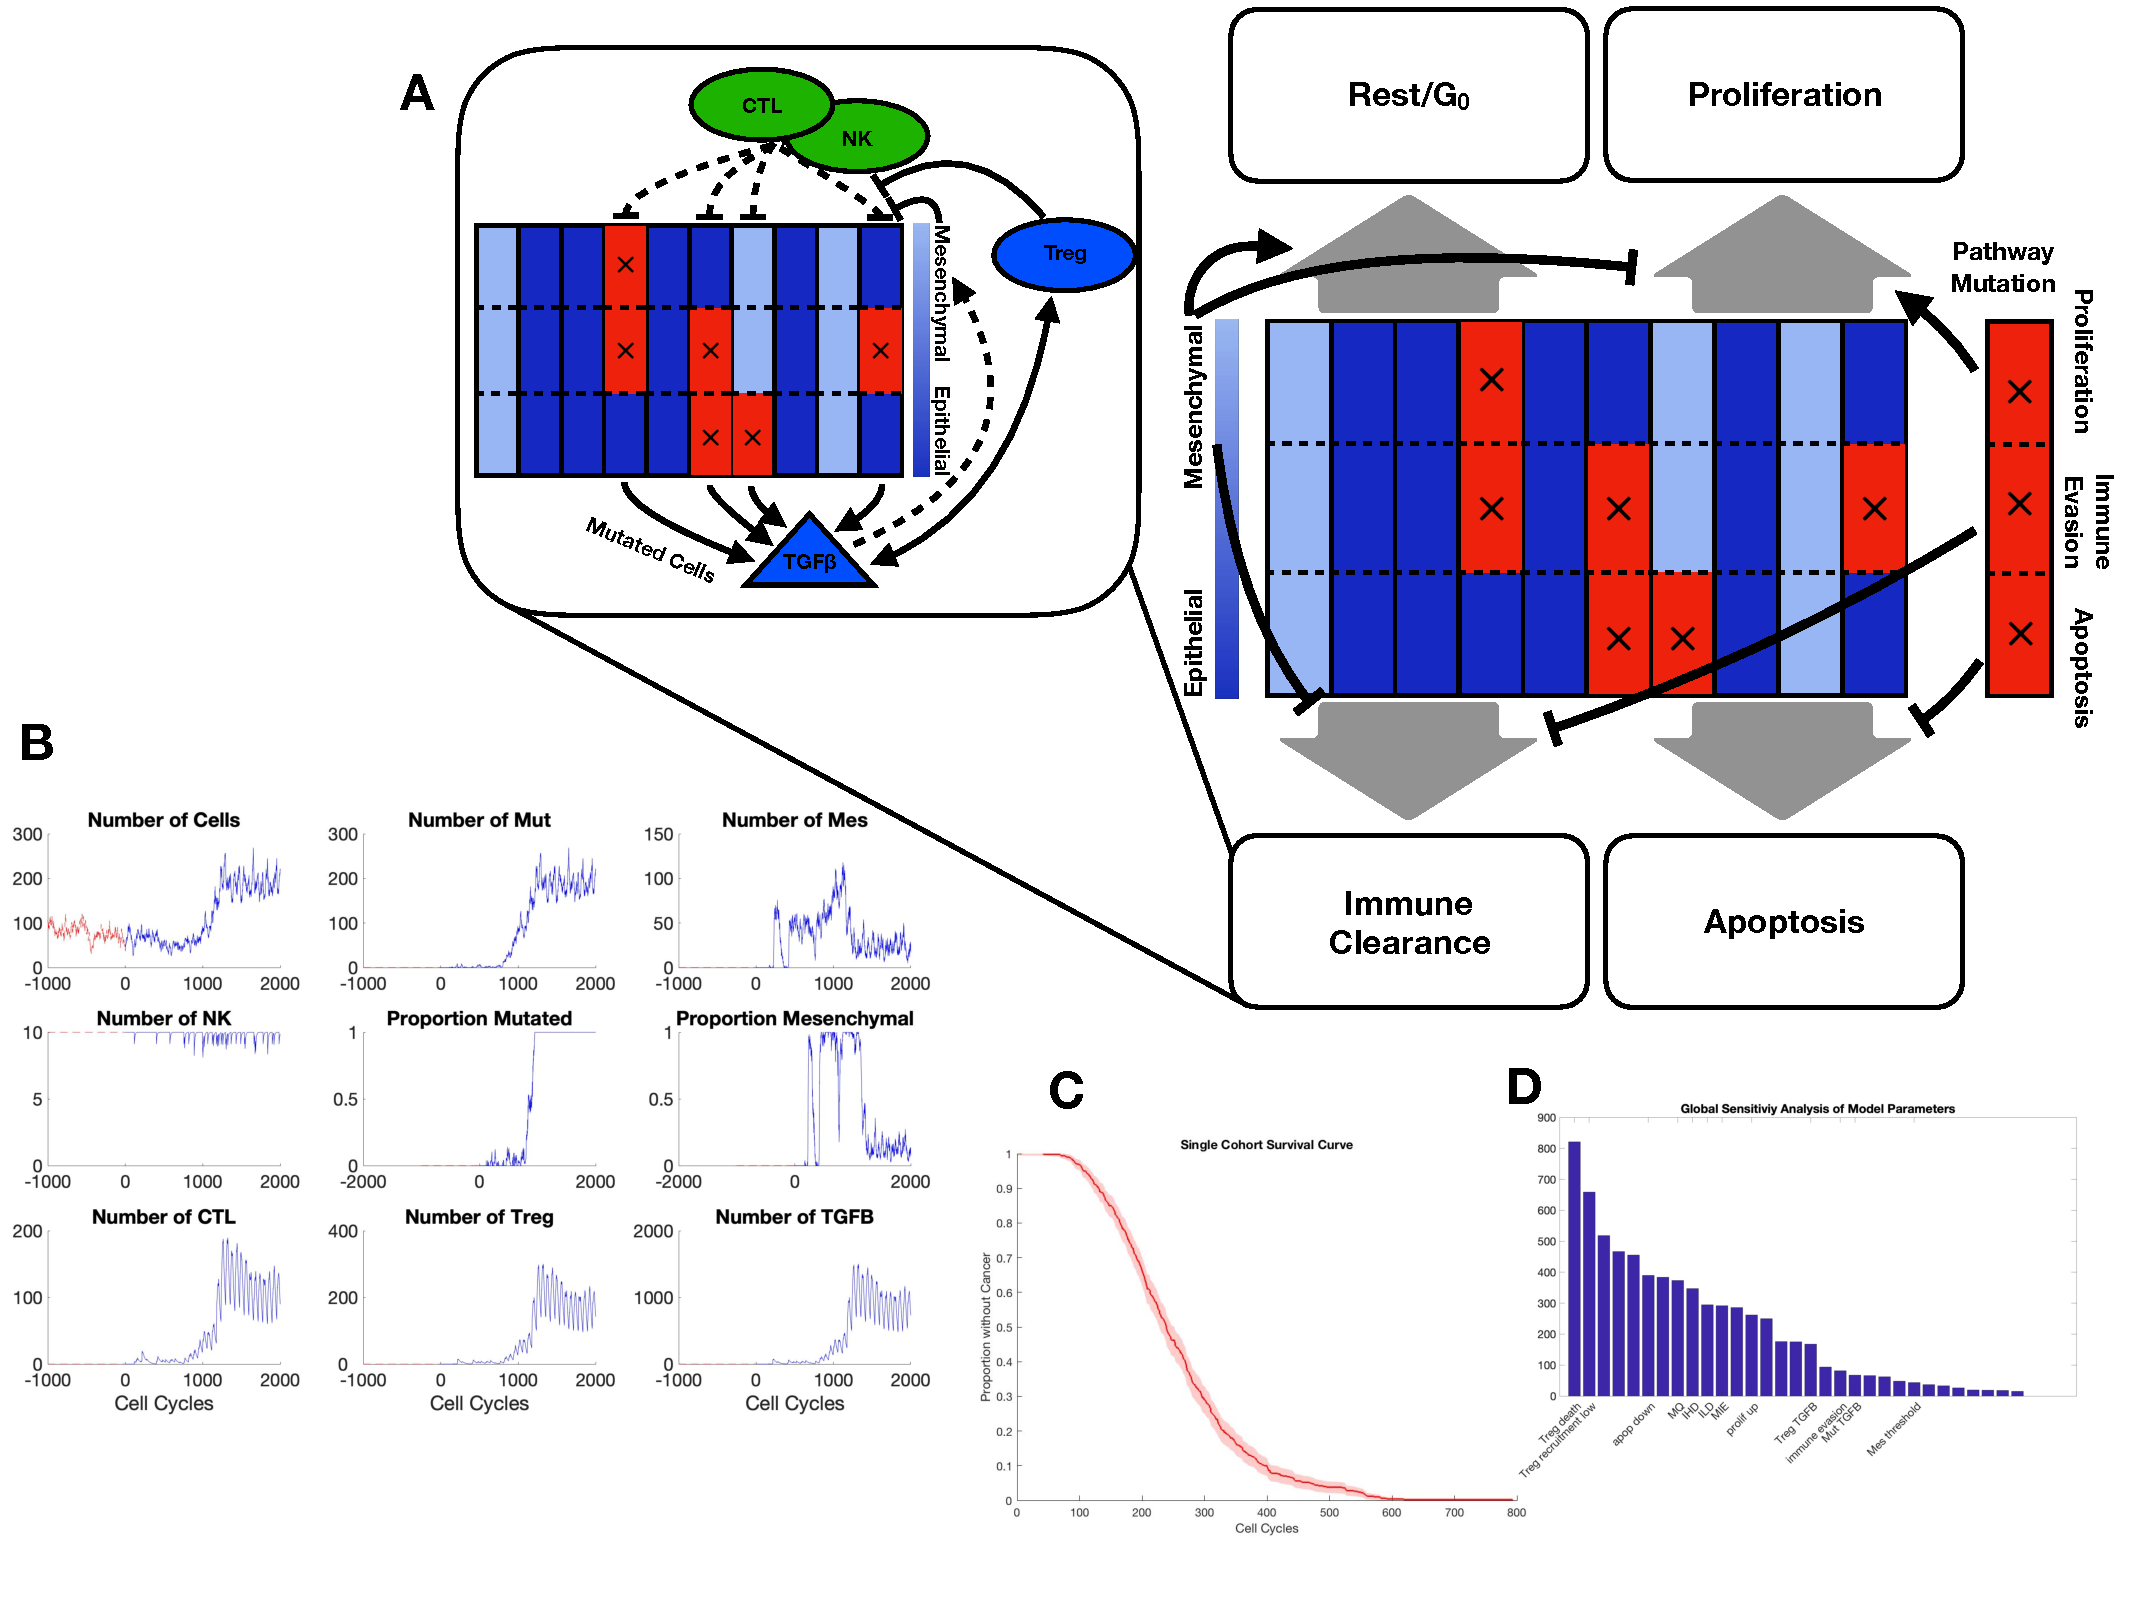
\includegraphics[width=0.9\textwidth]{Figure1/Figure1.pdf}}
\caption{A. Schematic depiction of agent-based model components; each of the 10 columns represents a single tumor cell divided into three compartments representing the state (altered or not) of the three pathways with mutagenic potential; red/blue denotes altered/unaltered pathways. Black arrows depict regulation of the cell fate in each cell cycle. Inset depicts major interactions between the immune system and tumor cells.
B. A representative simulation of one patient. The model parameter values used can be found in Table S2. 
The inflammation cycling scheme is represented above the patient dynamics. The vertical dashed line denotes the end of the warmup period. Mut: malignant cells; Mes: mesenchymal cells. 
C. Survival curve for one cohort of patients with the parameter values given in Table S2.}
\label{fig:ModelIntro}
\end{figure}

We begin by investigating general features of the model to establish baseline conditions and to assess the impact of various model components on the key measured outcomes: the probability of progression, and the Time to Cancer. 
Within the cell cycle, cell fate is determined via a set of rules that are influenced by EMT and immune interactions (Fig. \ref{fig:ModelIntro}A). For example, if a cell undergoes EMT, the probability that it will proliferate is reduced; if a cell gains a driver mutation in the apoptosis pathway, the probability that it undergoes apoptosis is greatly reduced.
The different means by which the immune system acts on tumor cells are also shown (\ref{fig:ModelIntro}A Inset). NK cells and CTLs attempt to clear malignant tumor cells, and deactivate upon successfully carrying out their cytotoxic function.
Tregs inhibit cytotoxic activity.
Tregs also release TGF-$\beta$ which promotes the recruitment of Tregs, as well as increasing the rate of EMT.
\par
The inflammation cycling scheme for a typical {\it in silico} patient consists of alternating high and low regimes (Fig. \ref{fig:ModelIntro}B); the inflammation schemes modeled will be discussed in detail in the next section.
For this patient, after the warmup period, cell mutations are observed at a rate low enough that they are cleared by cytotoxic cells before being able to establish a tumor.
After about 700 cell cycles, the malignant cell population begins to grow steadily.
At this point, large numbers of cells from the adaptive immune system (CTLs and Tregs) are being quickly recruited into the TME, and a peak in TGF-$\beta$ expression is observed.
After 841 cell cycles, the proportion of malignant cells reaches 50\%: the threshold defining progression.
Thus this patient has a Time to Cancer of 841 cell cycles, or 631 days.
For this patient, we kept let the simulation go beyond this timepoint, and we se that the number of malignant cells grows rapidly and soon makes up 100\% of the cell population.
A peak in number of mesenchymal cells is observed shortly after this threshold is reached, and following this most cells transition back to epithelial.
\par 
Considering the immune system dynamics, we see that the NK population is approximately constant, while the adaptive populations (CTL and Treg cells) grow quickly and dwarf NK cells in number following the accumulation of driver mutations.
The adaptive immune populations also appear to exhibit oscillatory behavior, however note that this is not due to intrinsic dynamics but rather due to the inflammation scheme that the patient is undergoing: alternating between 30 cell cycles of high inflammation and 60 cell cycles of low inflammation. Within each of these periods, adaptive immune populations increase or decrease rapidly in accordance with the inflammation state.
\par 
The {\em in silico} patient described here is given for the purpose of illustrating features of the model. Given the multiple sources of noise in the model, in order to quantify patient dynamics and cancer-free survival rates, below we will simulate large cohorts of patients. In Fig. \ref{fig:ModelIntro}C we simulate the survival curve for a cohort of $500$ patients: we see that all the patients survive for approximately 100 cell cycles (75 days). Subsequently, in the approximate range of $T= [100,300]$, the cancer onset rate is roughly constant, and after $600$ cell cycles, no patients remain cancer free.


\subsection{Identifying regulatory parameters via Morris global sensitivity analysis}\label{SensAnalysis}
Exploring the parameter spaces of models in systems biology is -- in general -- a hard problem. Performing Bayesian parameter inference to inform parameter values is advisable wherever possible \cite{kirk13_model}. Here, a lack of detailed molecular measurements  (i.e. data for tumor growth dynamics abound, but simultaneous data on the immune dynamics are lacking) preclude inference of the full model. In addition, while inference schemes for agent-based models are developing \cite{gallaher17_hybrid, warne19_simulation}, simulation times remain a hurdle \cite{lambert18_bayesian}. Parameters for aspects of this model that were studied previously can be constrained \cite{guo17_multiscale}, however even for these, the new additions to the model could push it into new behavioral regimes. Thus to adequately sample the parameter space of the model and identify those areas of parameter space that exert the most control, we use sensitivity analysis.   
\par
To assess the sensitivity of the model parameters and thus identify those that are most important in determining cancer-free survival times, we performed Morris one-step-at-a-time (OAT) sensitivity analysis (see Methods). 
The results of Morris OAT on the 31 model parameters are shown in Figure \ref{fig:MOAT}. We see that a subset of parameters demonstrate much higher levels of sensitivity than others.
The two most influential according to this analysis are the death rate and the recruitment rate of Treg cells, this is most likely due to the dual roles Treg cells play in both suppressing the cytotoxic effects of other immune cells and secreting TGF-$\beta$, which drives EMT.
This ties Treg cells to all three components of the model.
Since we seek to separate the effects of different model components, we do not choose the parameters influencing Treg cells for detailed analysis below.
\par 
Many parameters in the model change depending on the inflammation state.
For the sake of a naming convention, any parameter which includes ``low'' in the name represents the parameter value when inflammation is low.
For when the inflammation is high, these ``low'' parameters get scaled by parameters which include ``up'' in the name.
The ILD and IHD parameters determine the duration of low and high inflammation, respectively.
A cell with altered pathways will be affected by the $\Delta_A$, $\Delta_P$, and $\Delta_{\text{IE}}$ parameters, depending on whether the apoptosis, proliferation, or immune evasion pathways are altered.
The mesenchymal cells are influenced by the MGA and MIE parameters.
Finally, $\sigma$, $k_\text{EMT}$, $\tau_\text{max}$, and $K_3$ all control how cells transition between the epithelial and mesenchymal states.

Since one goal of our analysis is to assess the specific effects of EMT on immune-cancer dynamics, the parameters MIE and MGA are of particular interest.
In addition, inflammation parameters dictating the cycling scheme are of interest because they are both highly influential on Time to Cancer and capable of being targeted by therapeutic treatments.
In terms of Treg cells, their secretion of TGF-$\beta$ is highly significant and we will also study it further.


\begin{figure}
\center
{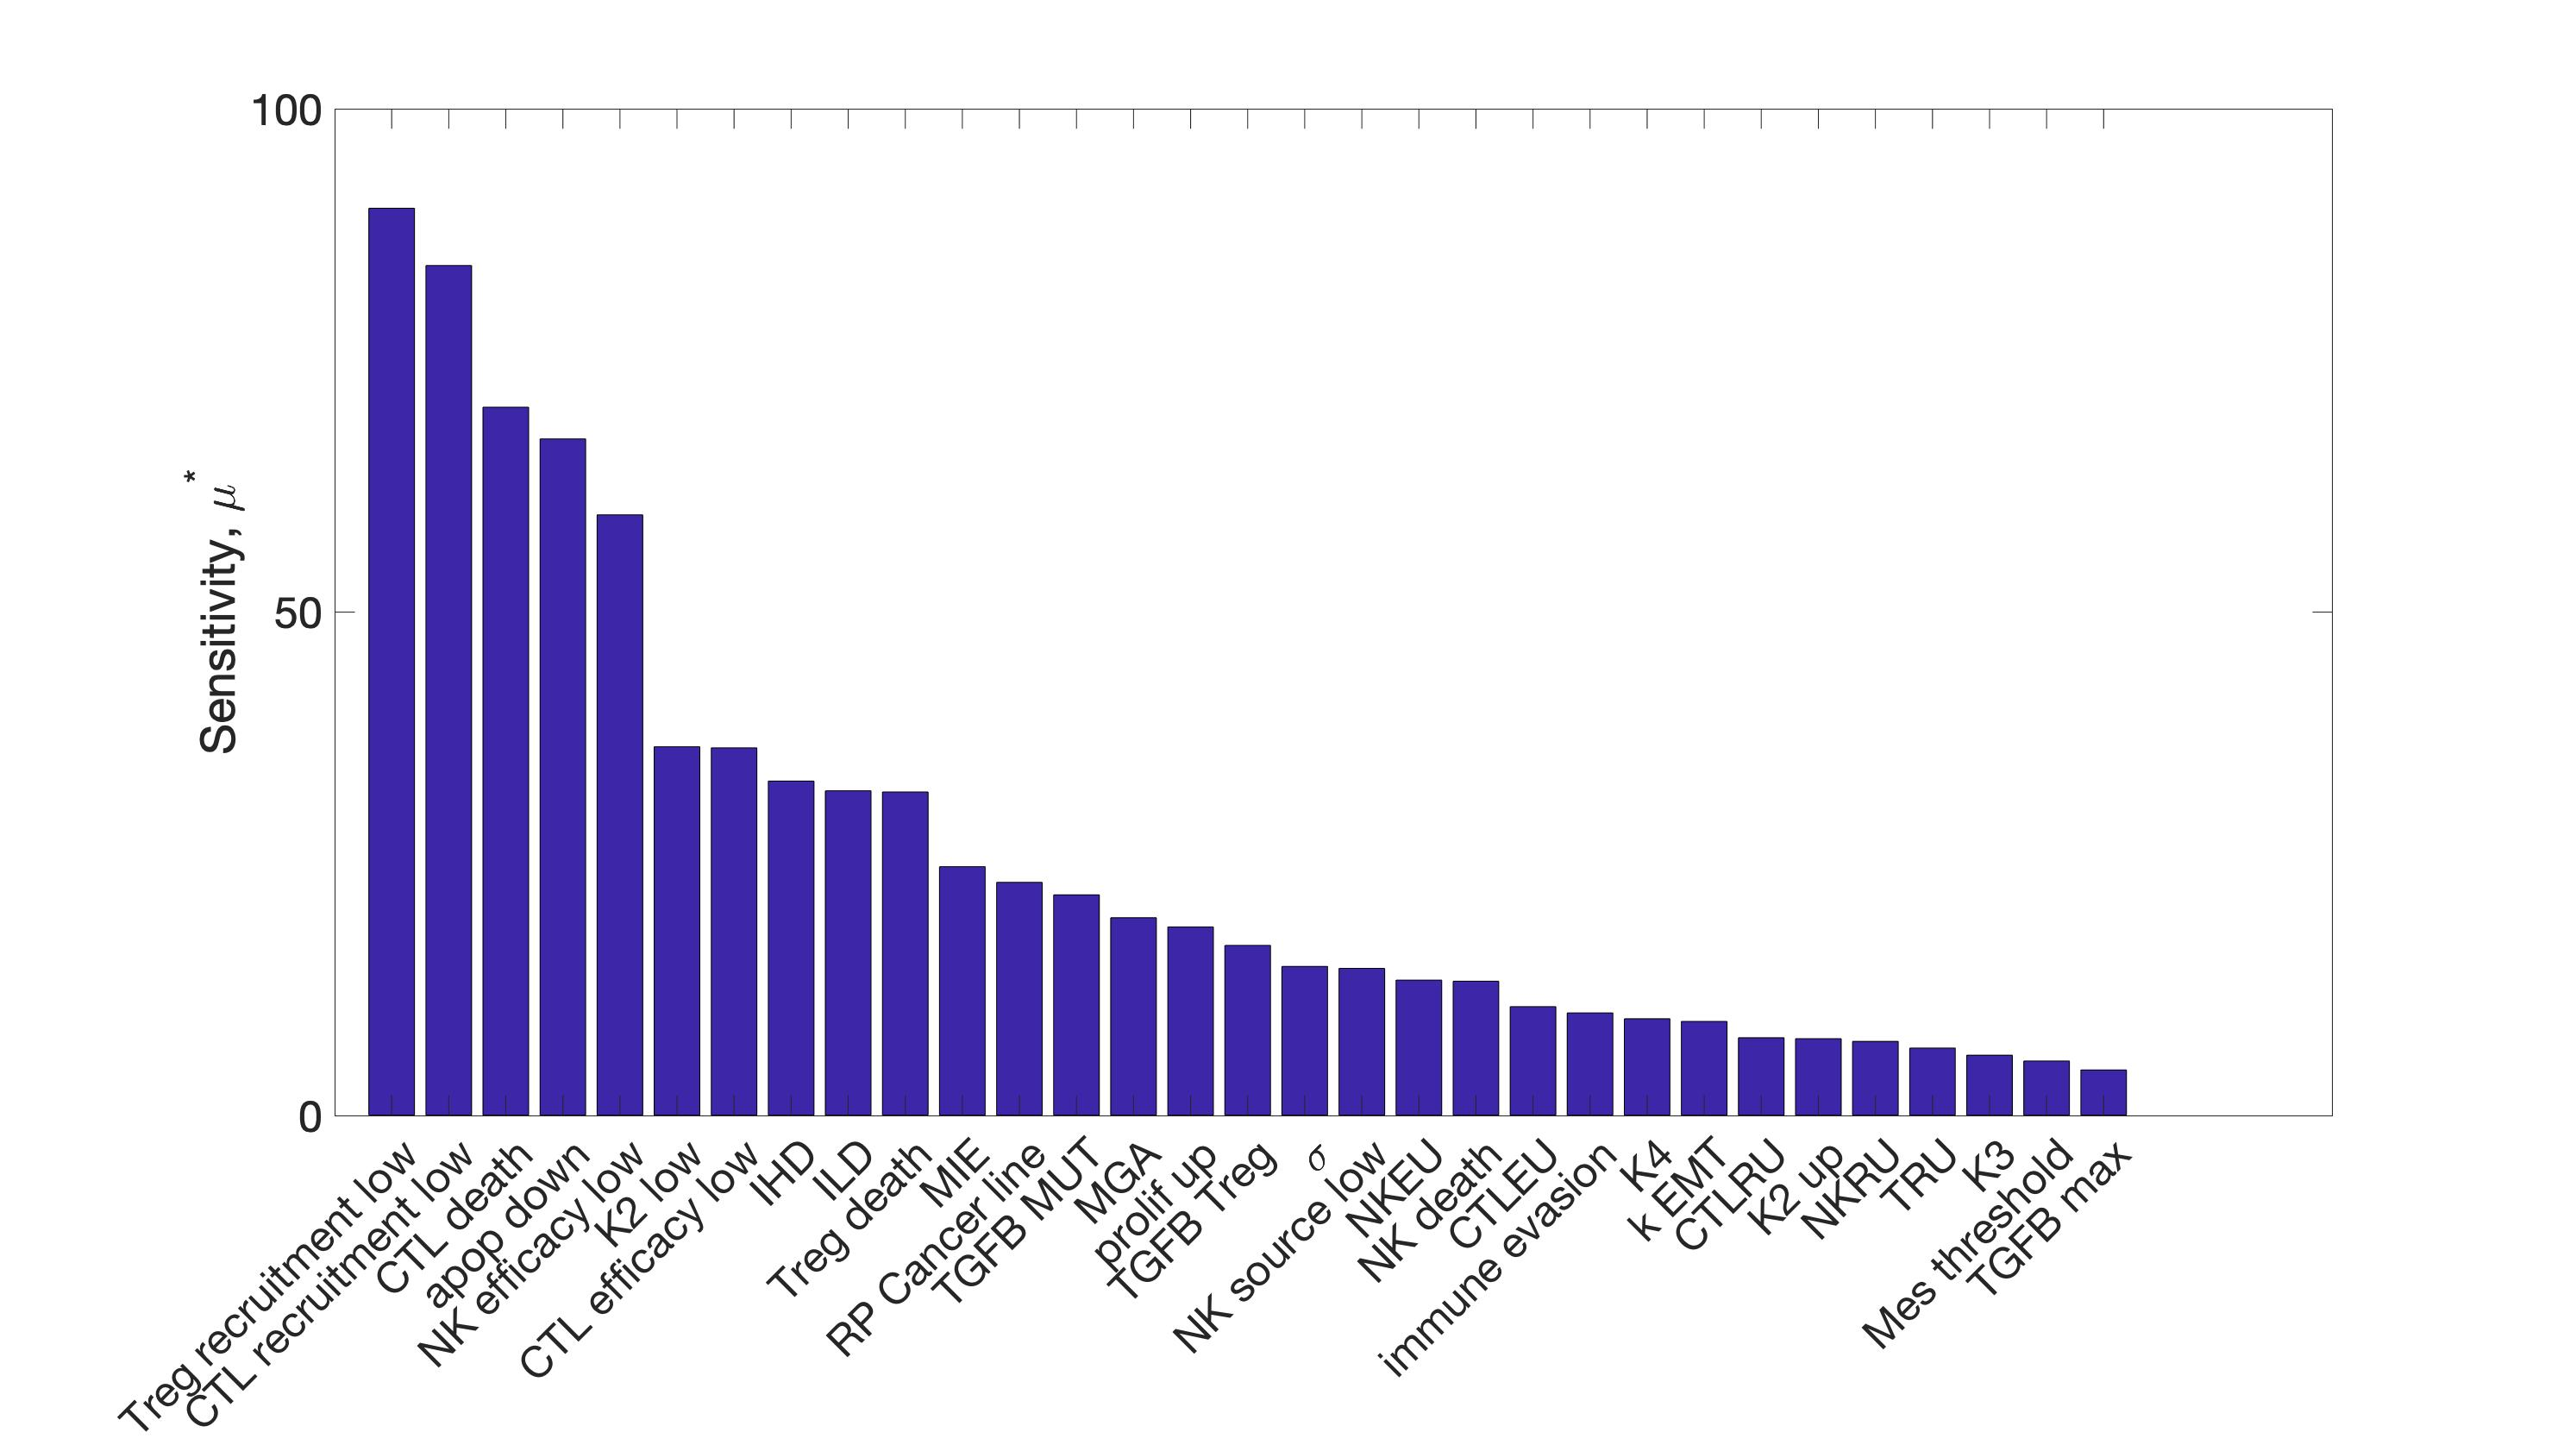
\includegraphics[width=0.85\textwidth]{Figure2/MOAT.jpg}}
\caption{Sensitivity analysis of model parameters, determined via the global Morris one-step-at-a-time method. $\mu^*$ denotes the average absolute change in Time to Cancer when the parameter is varied.}
\label{fig:MOAT}
\end{figure}

\subsection{Mesenchymal phenotypic properties dramatically alter invasion-free survival times}\label{MesPars}

\begin{figure}
\center
{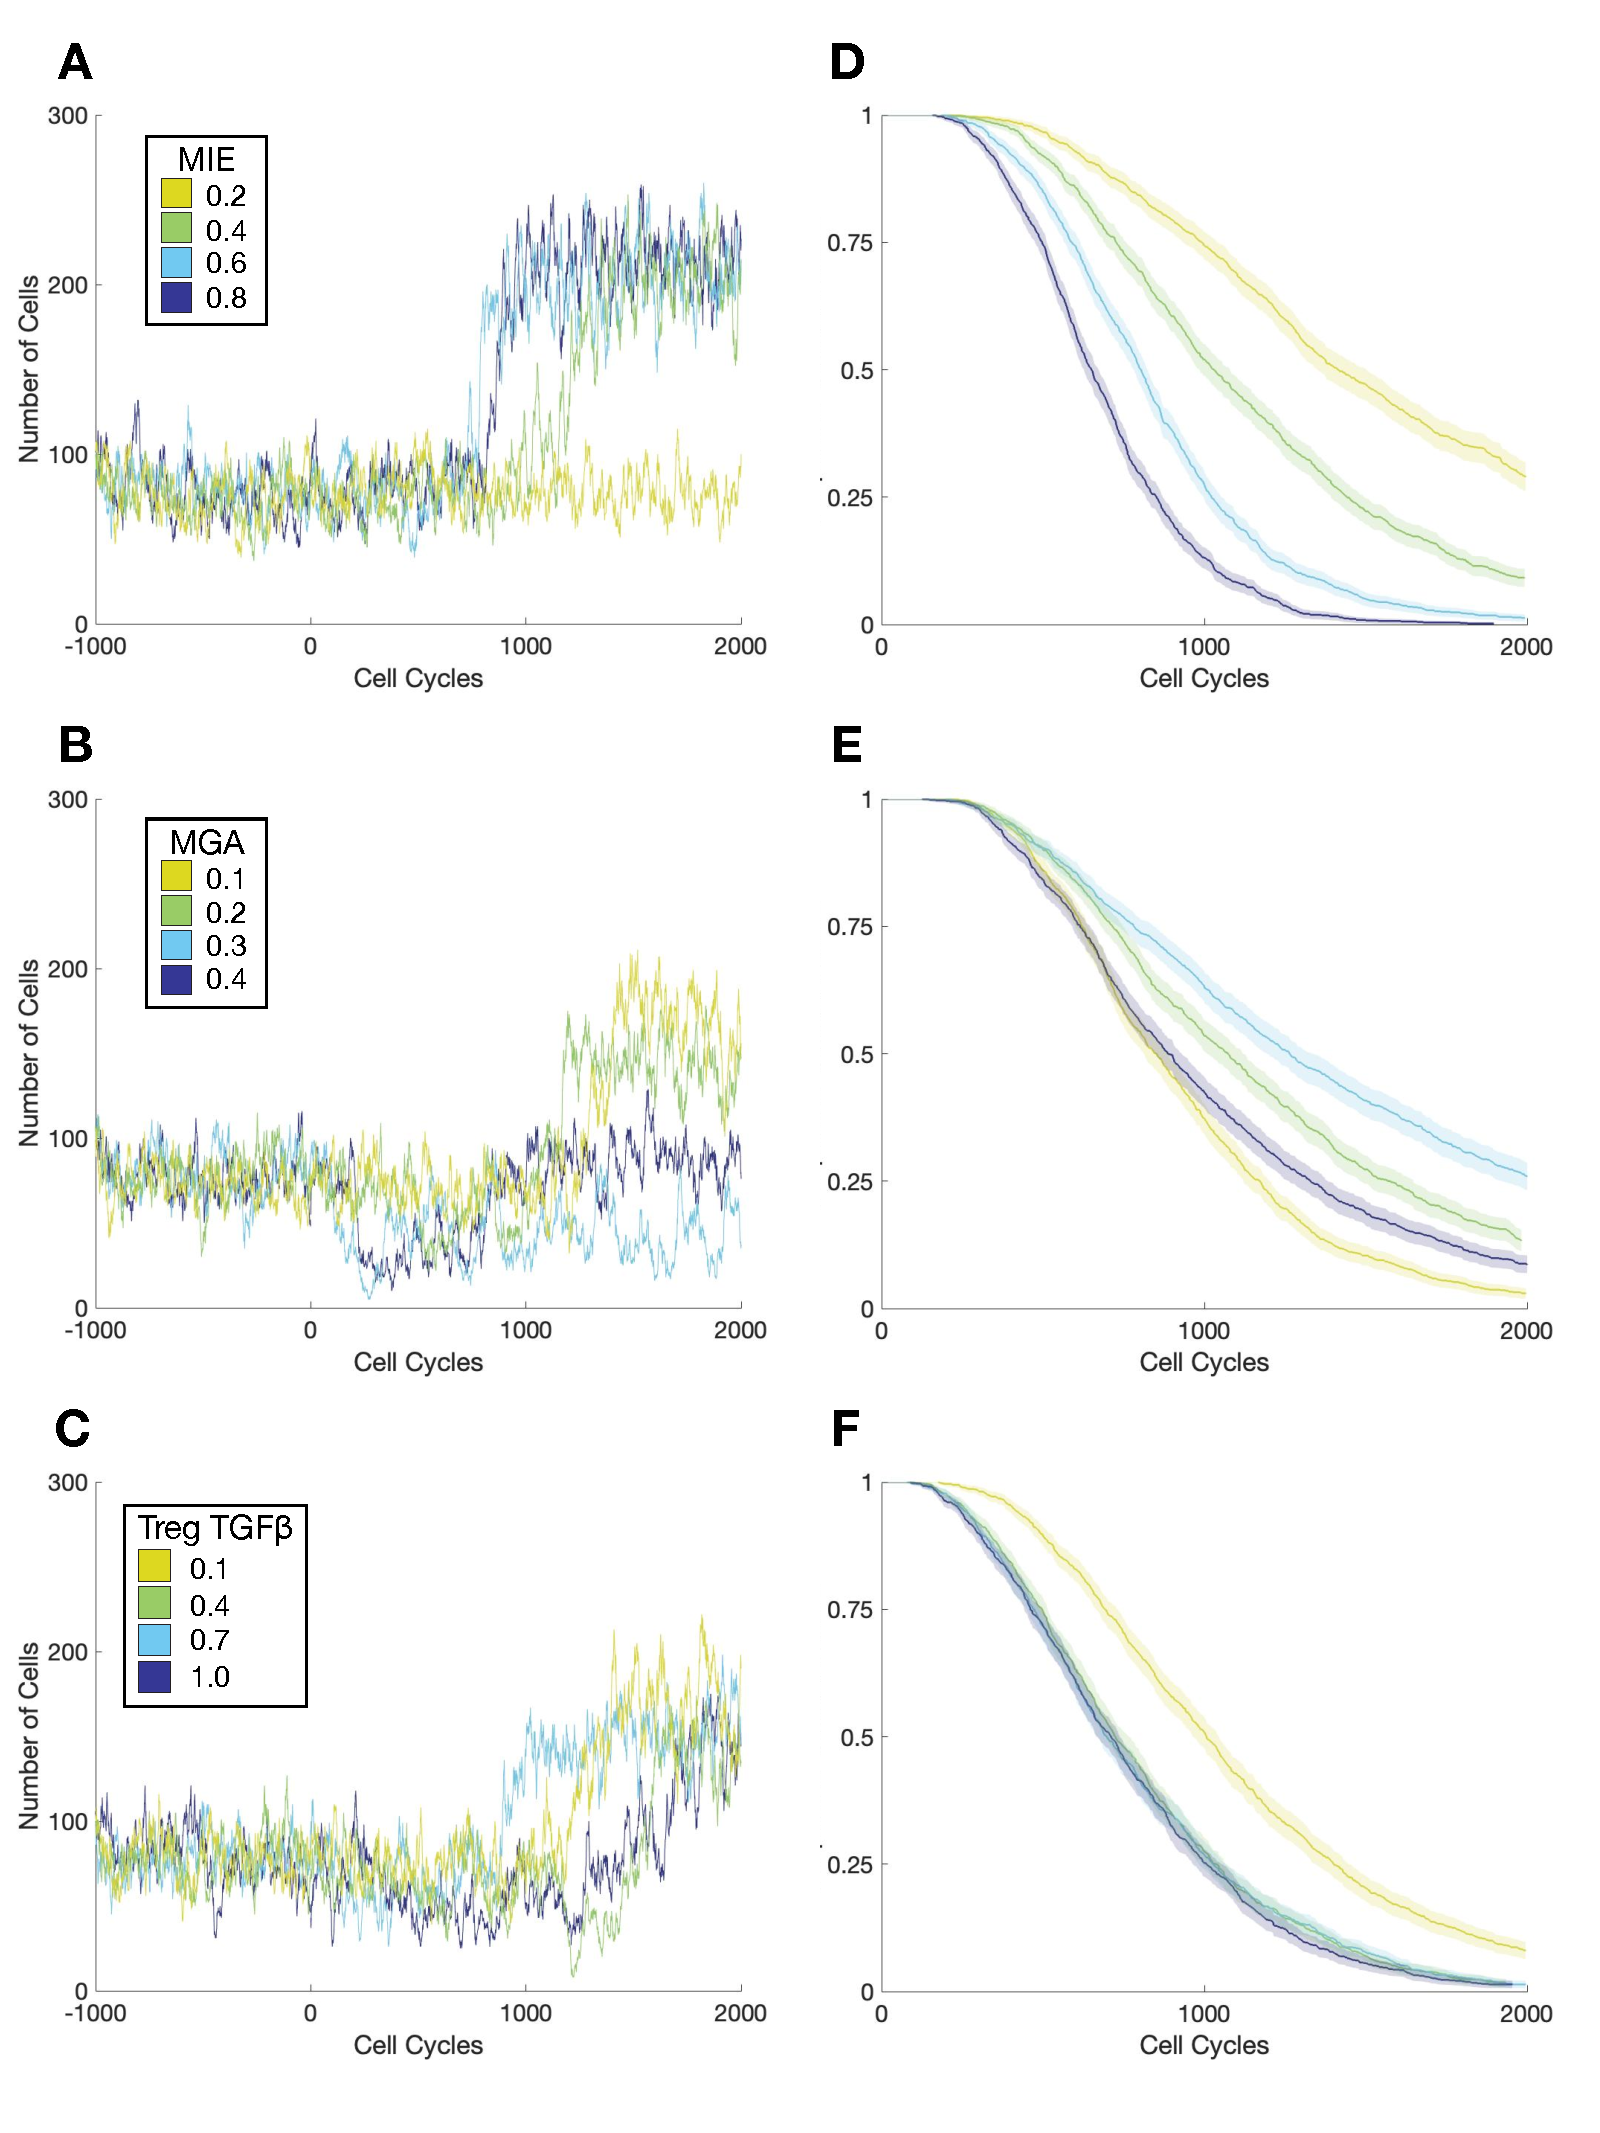
\includegraphics[width=0.85\textwidth]{Figure3/Figure3.pdf}}
\caption{Effects of mesenchymal tumor cell properties on the Time to Cancer. Trajectories of one patient per cohort from warmup period ([-1000,0]) to 2000 cell cycles, for $\Delta_\text{MIE}$ (A); $\Delta_\text{MGA}$ (B); and $\tau_\text{Treg}$ (C). 
D. Survival curves corresponding to changes in MIE (A) for a patient cohort of size 1000; shaded region represents the 95\% confidence interval for the evaluated function. 
E. Survival curves for patient cohort corresponding to changes in MGA (B).
F. Survival curves for patient cohort corresponding to changes in Treg TGF-$\beta$ (C). 
}
\label{fig:FirstSurvivalCurves}
\end{figure}


When a cell transitions from an epithelial to a mesenchymal state, two phenotypic cell characteristics change: mesenchymal immune evasion (MIE) and mesenchymal growth arrest (MGA).
Both parameters are defined proportionally, and lie in $[0,1]$, where higher values indicate more mesenchymal-like properties.
The parameter $\Delta_\text{MIE}$ is the proportional reduction in the probability that an invasive mesenchymal cell will be subject to immune clearance in a given cycle.
The parameter $\Delta_\text{MGA}$ is the proportional reduction in the probability that a mesenchymal cell will proliferate in a given cell cycle, thus is equivalent (strictly in terms of its impact on the cell cycle) to an increased proportion of time spent resting in the $G_0$ phase.
The cytokine TGF-$\beta$ is also involved in the EMT process (by increasing the probability of EMT). All three of these parameters were found to have large effects on the model by the Morris OAT analysis presented in Section \ref{SensAnalysis}.
\par 
As MIE increases, the invasion-free survival decreases (Fig. \ref{fig:FirstSurvivalCurves}A) under all sets of parameters studied: as this subpopulation of invasive cells becomes more resistant to immune clearance, the tumor as a whole grows more resilient and thus will grow faster.
These results are summarized by Fig. \ref{fig:FirstSurvivalCurves}A.
\par
As MGA increases, invasion-free survival increases: lower proliferation rates for mesenchymal cells slow down cancer progression (Fig \ref{fig:FirstSurvivalCurves}B).
This is not intuitive, since decreased proliferation rates affects all mesenchymal cells, not just the invasive cells.
\par
Third, TGF-$\beta$ can be varied in two ways: the production by mesenchymal cells and the production by Treg cells.
In Fig \ref{fig:FirstSurvivalCurves}C, the results of varying Treg TGF-$\beta$ production are shown, indicating that an increased Treg TGF-$\beta$ production leads to a shorter invasion-free survival time.
The two main ways in which TGF-$\beta$ influences the system is in recruitment of Treg cells and in pushing tumor cells to a mesenchymal phenotype.
Treg cells are modeled as tumor-protective and thus increasing their number will naturally decrease the invasion-free survival.
Mesenchymal cells are more likely to evade the immune system, so pushing the system towards an overall more mesenchymal state will lead to poorer outcomes, decreasing invasion-free survival times.

\begin{figure}
\center
{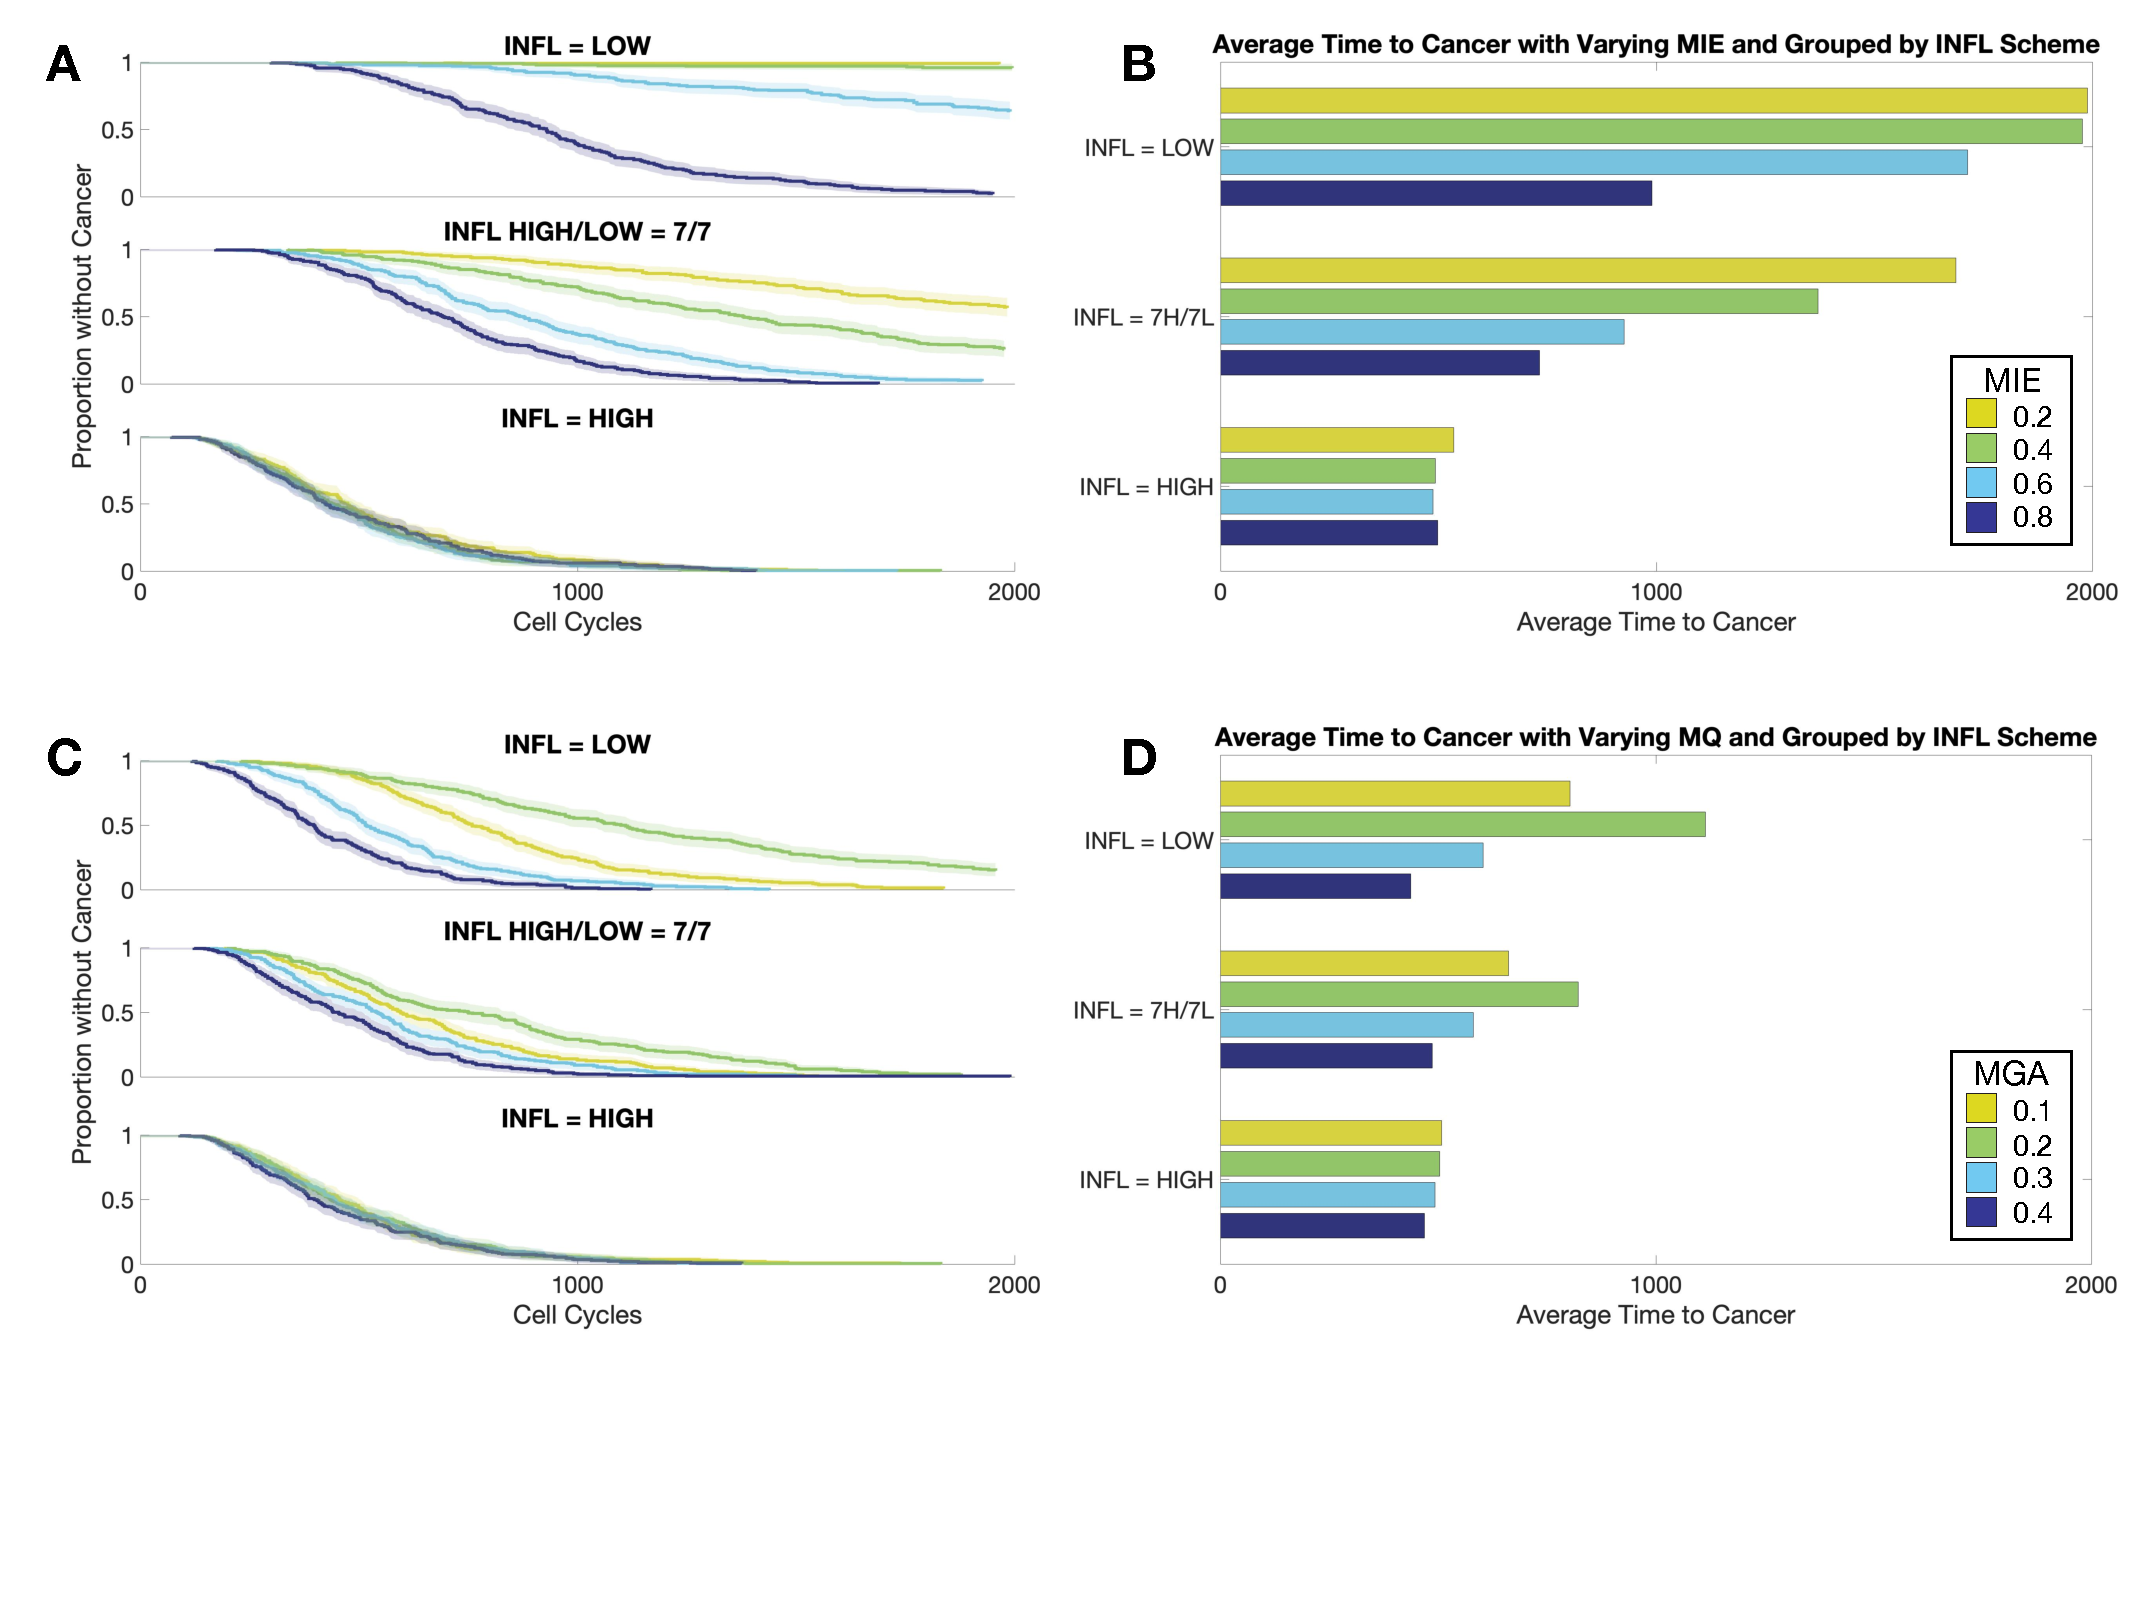
\includegraphics[width=0.95\textwidth]{Figure4/Figure4.pdf}}
\caption{Effects of inflammation on the Time to Cancer under different cycling schemes. A-B. As MIE varies, survival curves (each of 200 patients)  and corresponding bar plots to summarize the mean Time to Cancer for each cohort are shown. C-D. As MGA varies, survival curves  and corresponding bar plots to summarize the mean Time to Cancer for each cohort are shown.}
\label{fig:VaryINFL_and_MesPars}
\end{figure}

\subsection{A key EMT regime maximizes cancer-free survival time under chronic inflammation}\label{KeyEMT}

We explored the effects of varying the inflammation state of the patient on invasion-free survival, to investigate competing interactions within the tumor microenvironment and their effect on EMT. Patient cohorts were simulated under different inflammation regimes: permanently low inflammation; permanently high inflammation; or variable inflammation. For patients drawn from cohorts in a permanently high inflammatory state, the relationship between mesenchymal parameters and invasion-free survival is monotonic, i.e. increasing either MIE (Fig. \ref{fig:VaryINFL_and_MesPars}A-B) or MGA (Fig. \ref{fig:VaryINFL_and_MesPars}C-D) decreases the invasion-free survival time.
However, under regimes with either temporary or permanent periods of low inflammation, different relationships emerge: a local maximum for the invasion-free survival time is found with respect to MGA ($\Delta_\text{MGA}= 0.3$). This is seen both for intermittent or low inflammation (Fig. \ref{fig:VaryINFL_and_MesPars}D). 
\par
These striking differences in the mean invasion-free survival -- that can be extended by up to one year by optimization of the mesenchymal growth arrest -- have clear therapeutic implications. 
Our model predicts that a patient suffering intermittent inflammatory attacks at the tumor site will benefit from controlling the proliferation of the mesenchymal cells.
\par
In contrast, when MIE is varied for different inflammation cycling schemes, regardless of the cycling scheme, increasing the MIE will decreases the invasion-free survival (worsen cancer progression and prognosis). In the case where the inflammatory state is permanently high, however, MIE has little effect on the invasion-free survival time. Thus under any inflammation regime with periods of low inflammation, reductions of any size in the rate of mesenchymal immune evasion lead to improved patient outcomes.

\begin{figure}
\center
{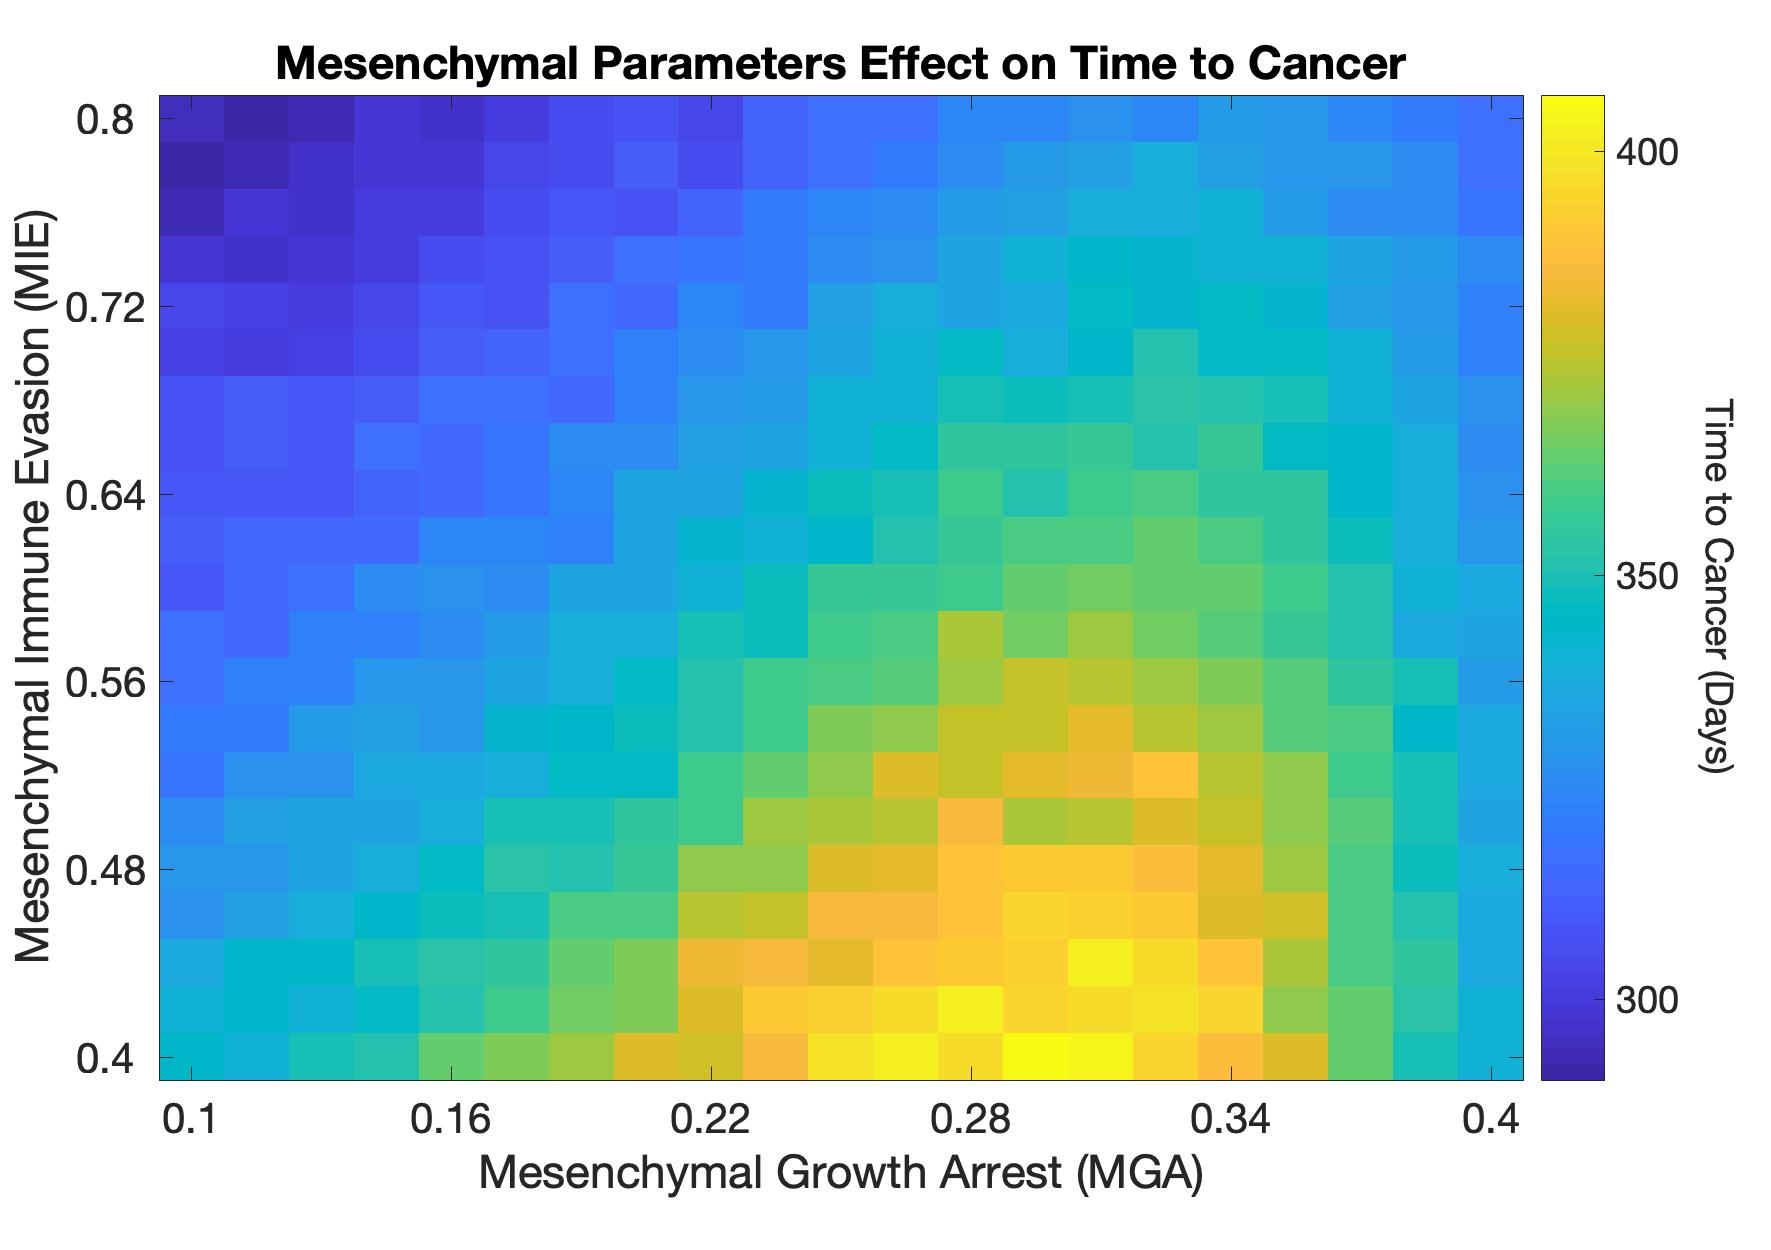
\includegraphics[width=0.5\textwidth]{Figure5/heatmap2.jpg}}
\caption{Summary of the contrasting effects of MIE and MGA on the Time to Cancer.
}
\label{fig:MIEvsMGA}
\end{figure}

\subsection{TCGA data analysis supports model predictions by showing that mesenchymal phenotypic properties reduce invasion-free survival }\label{tcga}

The effects that mesenchymal phenotypic properties have on progression can also be assessed by studying mesenchymal immune evasion ($\Delta_\text{MIE}$) and mesenchymal growth arrest ($\Delta_\text{MGA}$) on a heatmap (Fig. \ref{fig:MIEvsMGA}). We found that over the full range of values of $\Delta_\text{MGA}$ considered, increasing $\Delta_\text{MIE}$ decreases the invasion-free survival time. However, for any given value of mesenchymal immune evasion, there is a value of mesenchymal growth arrest that maximizes the invasion-free survival. Moreover, this optimal value increases with increasing MIE. Together these results show that while reducing the ability of a mutated cell to evade the immune system by any amount will improve the probability of invasion-free survival, an optimal value of MGA will prolong the tumor remaining in situ. 
\par
To compare these model predictions with experimental studies, we analyzed data from The Cancer Genome Atlas (TCGA) database to study the effects of immune and EMT interactions on prognosis of cancers for which inflammation is known to play an important role, such as colonic or pancreatic cancers \cite{greten2019inflammation,hu2010inflammation}.
The TCGA Pan-Cancer Clinical Data Resource (TCGA-CDR) provides multiple computed clinical endpoints for PAAD \cite{liu2018integrated}.
Here, we focus on the disease-free interval (DFI) and the overall survival (OS) endpoints.
In essence, a tumor where the DFI is short will undergo rapid (post-treatment) initiation.
In turn, we expect the distance between DFI and OS to be relatively small for a tumor undergoing rapid progression following initial (post-treatment) detection.
Therefore, recurrent tumors may be roughly categorized as either rapidly progressing or slowly progressing by defining a threshold for the DFI/OS divergence.
We selected three tumor types whose TCGA-CDR profile indicated slow progression (OV, SKCM, LIHC) and three tumor types whose profile indicated rapid progression (PAAD, LUAD, COAD).
See Figures \ref{fig:OV} and \ref{fig:PAAD} for OV and PAAD. The others will be in the supplement.
\par
For each cohort of cancer patients, we cluster the patients via k-means (n = 2) on gene ontologies relating to only EMT (Figures \ref{fig:OV}C, \ref{fig:PAAD}C), only inflammation (Figures \ref{fig:OV}E, \ref{fig:PAAD}E), and both EMT and inflammation (Figures \ref{fig:OV}A, \ref{fig:PAAD}A).
We also plot the corresponding survival curves for each of the clusters obtained (utilizing the originally reported OS endpoint).
We see that in both cases, survival is affected by the gene ontology signature, but the presence of both EMT and inflammatory signatures has a greater impact on survival than the effects of EMT alone.
This suggests that when studying interactions between cancer and the immune system, is it important to consider EMT; the effects of which may impact the dynamics and should not be overlooked. 


We note that the comparison between simulation and data here is indirect since the model studies the progression of cancer from an arbitrary starting point, while the data address the progression of cancer following treatment, but analogous processes are at play during both the progression of  clonal dynamics addressed by the model, and the progression of disease after cancer treatment.
In particular, the plasticity of tumor cells allows them to evade treatment by undergoing post-treatment processes resembling the de-novo appearance of cancer\cite{sanchez2018slow}.



\begin{figure}
\center
{\includegraphics[width=0.65\textwidth]{Figure6/OV.pdf}}
\caption{A. K-means clustering of OV using gene ontology terms indicative of EMT and inflammation signatures ($k=2$).
B. Survival plots corresponding to the clustering on EMT and inflammation.
C. K-means clustering of OV using gene ontology terms indicative of an EMT signature ($k=2$).
D. Survival plots corresponding to the clustering on EMT.
E. K-means clustering of OV using gene ontology terms indicative of inflammation ($k=2$).
F. Survival plots corresponding to the clustering on inflammation.}
\label{fig:OV}
\end{figure}

\begin{figure}
\center
{\includegraphics[width=0.65\textwidth]{Figure6/PAAD.pdf}}
\caption{A. K-means clustering of PAAD using gene ontology terms indicative of EMT and inflammation signatures ($k=2$).
B. Survival plots corresponding to the clustering on EMT and inflammation.
C. K-means clustering of PAAD using gene ontology terms indicative of an EMT signature ($k=2$).
D. Survival plots corresponding to the clustering on EMT.
E. K-means clustering of PAAD using gene ontology terms indicative of inflammation ($k=2$).
F. Survival plots corresponding to the clustering on inflammation.}
\label{fig:PAAD}
\end{figure}

%%%%%%%%%%%%%%%%%%%%%%%
%                      DISCUSSION                       %
%%%%%%%%%%%%%%%%%%%%%%%

\section{Discussion}\label{Discussion}
Despite the intense research focus on interactions between cancer and the immune system, and well as on the effects of EMT on cancer, there has not previously, to the best of our knowledge, been a model developed that combines these three components. Here we studied cancer, the immune system, and EMT, during the progression from an in situ tumor to invasive disease. We saw this as an even more pressing need given the shared factors that influence all of these, such as TGF-$\beta$. We used an individual cell-based model framework to describe the multiscale processes that can lead to cancer: DNA damage occurs during the cell cycle and this can lead to driver mutations in pathways that affect the fitness of the cell, which in turn affects the cell population dynamics, which are also influenced by the intrinsic state of the cell (EMT), and extrinsic immune factors (inflammation, cytotoxic cells, etc).
\par
We found that this model recapitulated invasion-free survival dynamics, and via global parameter sensitivity analysis, we identified parameters exerting key control over model behavior. Focusing on these led us to identify that: increasing mesenchymal immune evasion, decreasing mesenchymal growth arrest, or increasing Treg TGF-$\beta$ production all lead to shorter invasion-free survival times. However, varying the level of inflammation led to paradoxical effects: under regimes with periods of low inflammation, an optimal level of mesenchymal growth arrest can improve outcomes and maximize the invasion-free survival.
\par
To test these predictions, we performed unsupervised analysis of pancreatic cancer data from The Cancer Genome Atlas, and looked at survival across two groups: we found that the presence of an EMT signature increased differences in survival between groups in combination with inflammation. We chose to summarize {\em in silico} patient simulations with a single parameter: the invasion-free survival time, which we found captured the essential characteristics of the model. There are, of course, many tissue trajectories that all result in cancer, and it is our opinion that analysis of the transient cell dynamics in premalignant tissues is a pressing need to shed insight into cellular biomarkers of cancer.
\par
These results represent promising steps in understanding the competing roles of the immune system and EMT during progression of epithelial cancers, yet much remains to be done. Further development of the inflammation module of this model is important given the large and sometimes paradoxical roles that the inflammatory state exerts on the epithelia and cancer-free survival (Figs. \ref{fig:MOAT} and \ref{fig:VaryINFL_and_MesPars}B, D). Currently, inflammation is modeled as independently cycling between high and low schemes, however many of the agents considered in the model actively contribute to the inflammatory state, thus as an extension these components could be coupled, for example by assuming that the level of inflammation depends on the number of and the degree of mutations that cells in the tumor harbor).
%% not sure about
Another layer of complexity is revealed by the natural anti-inflammatory role of Tregs. One consequence of the current model is that decreasing the number of Tregs increases the cancer-free survival. Clearly, there exists a trade-off to be accounted for, and adding to the model the main effector function of Tregs could remedy this and add depth to our understanding of the various roles that Tregs play in and around the tumor.
\par
The roles that TGF-$\beta$ plays throughout the tumor and its microenvironment also warrant further investigation. We found that, below a certain threshold, reduction of TGF-$\beta$ increases the Time to Cancer  (Fig. \ref{fig:FirstSurvivalCurves}E), thus reducing expression levels of TGF-$\beta$ in the tumor microenvironment benefits survival. Intriguingly, recent experimental work demonstrated that TGF-$\beta$ drives tumor suppression in pancreatic cancer by promoting EMT \cite{david16_tgfv}. However, TGF-$\beta$ is a master regulator implicated in numerous cellular signaling processes, and changing the concentrations of TGF-$\beta$ even in a local tumor microenvironment could have large off-target effects. Indeed, it has been showns that TGF-$\beta$ promotes invasion and heterogeneity (although suppresses cell proliferation) in squamous cell carcinoma \cite{oshimori15_tgfv}. Future work thus ought to consider the effects of targeting signaling factors downstream of TGF-$\beta$ that still have the ability to modulate epithelial cell dynamics. Towards this end, we are currently developing a larger TGF-$\beta$ signaling pathway module with appropriate crosstalks to  epithelial/mesenchymal/immune cell functions to be incorporated into the model.
\par
A further goal for future work is to explore (and exploit) the heterogeneity of tumor evolution in greater depth: this heterogeneity aids the evasion of the tumor from immune effects. Studying the consequences of decanalization \cite{gibson09_decanalization} during cancer progression is too-often sidelined, despite evidence supporting its prominence \cite{cyll17_tumour, punt17_tumour, dagogo-jack18_tumour}. Yet despite these challenges, for which the complexity of the disease may be often in large part responsible, great progress has been and continues to be made. As we approach a new generation of immunotherapies, it is these very complexities that we must better understand in order to control or eradicate the disease.

\section*{Acknowledgements}
Q.N. would like to acknowledge partial support for this work from National Institutes of Health grants R01GM123731, U01AR073159, and U54-CA217378; National Science Foundation grants DMS1562176 and DMS1763272; Simons Foundation grant (594598); and the Jayne Koskinas Ted Giovanis Foundation for Health and Policy joint with the Breast Cancer Research Foundation. A.L.M. would like to acknowledge partial support for this work from the American Cancer Society grant \#IRG-16-181-57.


\bibliography{mybib,amrefs}
\bibliographystyle{plos2015}

\end{document}
